% Options for packages loaded elsewhere
\PassOptionsToPackage{unicode}{hyperref}
\PassOptionsToPackage{hyphens}{url}
%
\documentclass[
]{article}
\usepackage{lmodern}
\usepackage{amssymb,amsmath}
\usepackage{ifxetex,ifluatex}
\ifnum 0\ifxetex 1\fi\ifluatex 1\fi=0 % if pdftex
  \usepackage[T1]{fontenc}
  \usepackage[utf8]{inputenc}
  \usepackage{textcomp} % provide euro and other symbols
\else % if luatex or xetex
  \usepackage{unicode-math}
  \defaultfontfeatures{Scale=MatchLowercase}
  \defaultfontfeatures[\rmfamily]{Ligatures=TeX,Scale=1}
\fi
% Use upquote if available, for straight quotes in verbatim environments
\IfFileExists{upquote.sty}{\usepackage{upquote}}{}
\IfFileExists{microtype.sty}{% use microtype if available
  \usepackage[]{microtype}
  \UseMicrotypeSet[protrusion]{basicmath} % disable protrusion for tt fonts
}{}
\makeatletter
\@ifundefined{KOMAClassName}{% if non-KOMA class
  \IfFileExists{parskip.sty}{%
    \usepackage{parskip}
  }{% else
    \setlength{\parindent}{0pt}
    \setlength{\parskip}{6pt plus 2pt minus 1pt}}
}{% if KOMA class
  \KOMAoptions{parskip=half}}
\makeatother
\usepackage{xcolor}
\IfFileExists{xurl.sty}{\usepackage{xurl}}{} % add URL line breaks if available
\IfFileExists{bookmark.sty}{\usepackage{bookmark}}{\usepackage{hyperref}}
\hypersetup{
  hidelinks,
  pdfcreator={LaTeX via pandoc}}
\urlstyle{same} % disable monospaced font for URLs
\usepackage[margin=1in]{geometry}
\usepackage{color}
\usepackage{fancyvrb}
\newcommand{\VerbBar}{|}
\newcommand{\VERB}{\Verb[commandchars=\\\{\}]}
\DefineVerbatimEnvironment{Highlighting}{Verbatim}{commandchars=\\\{\}}
% Add ',fontsize=\small' for more characters per line
\usepackage{framed}
\definecolor{shadecolor}{RGB}{248,248,248}
\newenvironment{Shaded}{\begin{snugshade}}{\end{snugshade}}
\newcommand{\AlertTok}[1]{\textcolor[rgb]{0.94,0.16,0.16}{#1}}
\newcommand{\AnnotationTok}[1]{\textcolor[rgb]{0.56,0.35,0.01}{\textbf{\textit{#1}}}}
\newcommand{\AttributeTok}[1]{\textcolor[rgb]{0.77,0.63,0.00}{#1}}
\newcommand{\BaseNTok}[1]{\textcolor[rgb]{0.00,0.00,0.81}{#1}}
\newcommand{\BuiltInTok}[1]{#1}
\newcommand{\CharTok}[1]{\textcolor[rgb]{0.31,0.60,0.02}{#1}}
\newcommand{\CommentTok}[1]{\textcolor[rgb]{0.56,0.35,0.01}{\textit{#1}}}
\newcommand{\CommentVarTok}[1]{\textcolor[rgb]{0.56,0.35,0.01}{\textbf{\textit{#1}}}}
\newcommand{\ConstantTok}[1]{\textcolor[rgb]{0.00,0.00,0.00}{#1}}
\newcommand{\ControlFlowTok}[1]{\textcolor[rgb]{0.13,0.29,0.53}{\textbf{#1}}}
\newcommand{\DataTypeTok}[1]{\textcolor[rgb]{0.13,0.29,0.53}{#1}}
\newcommand{\DecValTok}[1]{\textcolor[rgb]{0.00,0.00,0.81}{#1}}
\newcommand{\DocumentationTok}[1]{\textcolor[rgb]{0.56,0.35,0.01}{\textbf{\textit{#1}}}}
\newcommand{\ErrorTok}[1]{\textcolor[rgb]{0.64,0.00,0.00}{\textbf{#1}}}
\newcommand{\ExtensionTok}[1]{#1}
\newcommand{\FloatTok}[1]{\textcolor[rgb]{0.00,0.00,0.81}{#1}}
\newcommand{\FunctionTok}[1]{\textcolor[rgb]{0.00,0.00,0.00}{#1}}
\newcommand{\ImportTok}[1]{#1}
\newcommand{\InformationTok}[1]{\textcolor[rgb]{0.56,0.35,0.01}{\textbf{\textit{#1}}}}
\newcommand{\KeywordTok}[1]{\textcolor[rgb]{0.13,0.29,0.53}{\textbf{#1}}}
\newcommand{\NormalTok}[1]{#1}
\newcommand{\OperatorTok}[1]{\textcolor[rgb]{0.81,0.36,0.00}{\textbf{#1}}}
\newcommand{\OtherTok}[1]{\textcolor[rgb]{0.56,0.35,0.01}{#1}}
\newcommand{\PreprocessorTok}[1]{\textcolor[rgb]{0.56,0.35,0.01}{\textit{#1}}}
\newcommand{\RegionMarkerTok}[1]{#1}
\newcommand{\SpecialCharTok}[1]{\textcolor[rgb]{0.00,0.00,0.00}{#1}}
\newcommand{\SpecialStringTok}[1]{\textcolor[rgb]{0.31,0.60,0.02}{#1}}
\newcommand{\StringTok}[1]{\textcolor[rgb]{0.31,0.60,0.02}{#1}}
\newcommand{\VariableTok}[1]{\textcolor[rgb]{0.00,0.00,0.00}{#1}}
\newcommand{\VerbatimStringTok}[1]{\textcolor[rgb]{0.31,0.60,0.02}{#1}}
\newcommand{\WarningTok}[1]{\textcolor[rgb]{0.56,0.35,0.01}{\textbf{\textit{#1}}}}
\usepackage{graphicx,grffile}
\makeatletter
\def\maxwidth{\ifdim\Gin@nat@width>\linewidth\linewidth\else\Gin@nat@width\fi}
\def\maxheight{\ifdim\Gin@nat@height>\textheight\textheight\else\Gin@nat@height\fi}
\makeatother
% Scale images if necessary, so that they will not overflow the page
% margins by default, and it is still possible to overwrite the defaults
% using explicit options in \includegraphics[width, height, ...]{}
\setkeys{Gin}{width=\maxwidth,height=\maxheight,keepaspectratio}
% Set default figure placement to htbp
\makeatletter
\def\fps@figure{htbp}
\makeatother
\setlength{\emergencystretch}{3em} % prevent overfull lines
\providecommand{\tightlist}{%
  \setlength{\itemsep}{0pt}\setlength{\parskip}{0pt}}
\setcounter{secnumdepth}{-\maxdimen} % remove section numbering

\author{}
\date{\vspace{-2.5em}}

\begin{document}

\section{Appendix B: R Code for Chapter 4}
\label{sec:Appendix B: R Code for Chapter 4}

\singlespace

Required: R Packages from CRAN (in addition to packages already found in
Chapter 3)

\small

\begin{Shaded}
\begin{Highlighting}[]
\ControlFlowTok{if}\NormalTok{ (}\OperatorTok{!}\KeywordTok{require}\NormalTok{(MuMIn))\{}
  \KeywordTok{install.packages}\NormalTok{(}\StringTok{"MuMIn"}\NormalTok{)}
  \KeywordTok{library}\NormalTok{(MuMIn)}
\NormalTok{\}}
\ControlFlowTok{if}\NormalTok{ (}\OperatorTok{!}\KeywordTok{require}\NormalTok{(parallel))\{}
  \KeywordTok{install.packages}\NormalTok{(}\StringTok{"parallel"}\NormalTok{)}
  \KeywordTok{library}\NormalTok{(parallel)}
\NormalTok{\}}
\ControlFlowTok{if}\NormalTok{ (}\OperatorTok{!}\KeywordTok{require}\NormalTok{(R2HTML))\{}
  \KeywordTok{install.packages}\NormalTok{(}\StringTok{"R2HTML"}\NormalTok{)}
  \KeywordTok{library}\NormalTok{(R2HTML)}
\NormalTok{\}}
\ControlFlowTok{if}\NormalTok{ (}\OperatorTok{!}\KeywordTok{require}\NormalTok{(e1071))\{}
  \KeywordTok{install.packages}\NormalTok{(}\StringTok{"e1071"}\NormalTok{)}
  \KeywordTok{library}\NormalTok{(e1071)}
\NormalTok{\}}
\ControlFlowTok{if}\NormalTok{ (}\OperatorTok{!}\KeywordTok{require}\NormalTok{(ROCR))\{}
  \KeywordTok{install.packages}\NormalTok{(}\StringTok{"ROCR"}\NormalTok{)}
  \KeywordTok{library}\NormalTok{(ROCR)}
\NormalTok{\}}
\end{Highlighting}
\end{Shaded}

\normalsize

\subsection{Data partitioning of the pre-processed OpRisk dataset into Training/Validation/Testing proportions, in preparation for machine learning model building treatments. The original dataset is partitioned into three random subsets initiated by a random number sequence with a randomly selected seed.}
\label{ssec:Data Training/Validation/Testing}

The function \texttt{getmode} specifies the modal class as the reference
level in the GLM from which the corresponding observations are estmated
and weighted against, see chapter
\ref{DATA EXPLORATION AND EXPOSURE VARIABLE ANALYSIS} section
\ref{sec:Exploratory data analysis} on page
\pageref{sec:Exploratory data analysis}

\small

\begin{Shaded}
\begin{Highlighting}[]
\NormalTok{building <-}\StringTok{ }\OtherTok{TRUE}
\NormalTok{scoring <-}\StringTok{ }\OperatorTok{!}\StringTok{ }\NormalTok{building}

\CommentTok{# Load data}
\NormalTok{fname <-}\StringTok{ "file:///C:/Users/Mphekeleli/Documents/R PROJECT/OpRiskPHDGitHub}
\StringTok{/OpRisk_PHD_Thesis/Data/OPriskDataSet_exposure.csv"}
\NormalTok{crs}\OperatorTok{$}\NormalTok{dataset <-}\StringTok{ }\KeywordTok{read.csv}\NormalTok{(fname,}
              \DataTypeTok{sep=}\StringTok{";"}\NormalTok{,}
              \DataTypeTok{dec=}\StringTok{","}\NormalTok{,}
              \DataTypeTok{na.strings=}\KeywordTok{c}\NormalTok{(}\StringTok{"."}\NormalTok{, }\StringTok{"NA"}\NormalTok{, }\StringTok{""}\NormalTok{, }\StringTok{"?"}\NormalTok{),}
              \DataTypeTok{strip.white=}\OtherTok{TRUE}\NormalTok{, }\DataTypeTok{encoding=}\StringTok{"UTF-8"}\NormalTok{)}
\NormalTok{exposure <-}\StringTok{ }\NormalTok{crs}\OperatorTok{$}\NormalTok{dataset[,}\KeywordTok{ncol}\NormalTok{(crs}\OperatorTok{$}\NormalTok{dataset)]}

\CommentTok{# Select variables for loss incident model}
\NormalTok{crs}\OperatorTok{$}\NormalTok{dataset <-}\StringTok{ }\KeywordTok{as.data.frame}\NormalTok{(crs}\OperatorTok{$}\NormalTok{dataset)}

\CommentTok{# The following varaible selections have been noted}

\NormalTok{crs}\OperatorTok{$}\NormalTok{input <-}\StringTok{ }\NormalTok{crs}\OperatorTok{$}\NormalTok{dataset }\OperatorTok
\StringTok{  }\KeywordTok{group_by}\NormalTok{(UpdatedDay,}
\NormalTok{           UpdatedTime,}
\NormalTok{           TradedDay,}
\NormalTok{           TradedTime,}
\NormalTok{           Desk,}
\NormalTok{           CapturedBy,}
\NormalTok{           TradeStatus,}
\NormalTok{           TraderId,}
\NormalTok{           Instrument,}
\NormalTok{           Reason,}
\NormalTok{           EventTypeCategoryLevel1,}
\NormalTok{           BusinessLineLevel1) }\OperatorTok
\StringTok{  }\KeywordTok{transmute}\NormalTok{(}\DataTypeTok{LossesIndicator =}\NormalTok{ LossIndicator,}
            \DataTypeTok{Losses =}\NormalTok{ Loss,}
            \DataTypeTok{Exposure =}\NormalTok{ exposure)}

\NormalTok{getmode <-}\StringTok{ }\ControlFlowTok{function}\NormalTok{(x)\{}
\NormalTok{  u <-}\StringTok{ }\KeywordTok{unique}\NormalTok{(x)}
  \KeywordTok{as.integer}\NormalTok{(u[}\KeywordTok{which.max}\NormalTok{(}\KeywordTok{tabulate}\NormalTok{(}\KeywordTok{match}\NormalTok{(x,u)))])}
\NormalTok{\}}

\ControlFlowTok{for}\NormalTok{ (i }\ControlFlowTok{in} \DecValTok{5}\OperatorTok{:}\NormalTok{(}\KeywordTok{ncol}\NormalTok{(crs}\OperatorTok{$}\NormalTok{input) }\OperatorTok{-}\StringTok{ }\DecValTok{3}\NormalTok{))\{}
\NormalTok{     crs}\OperatorTok{$}\NormalTok{input[[i]] <-}\StringTok{ }\KeywordTok{relevel}\NormalTok{(crs}\OperatorTok{$}\NormalTok{input[[i]], }\KeywordTok{getmode}\NormalTok{(crs}\OperatorTok{$}\NormalTok{input[[i]]))}
\NormalTok{\}}

\CommentTok{#==========================================================================================}
\CommentTok{# A predefined value is used to reset the random seed so that results are repeatable}
\NormalTok{crv}\OperatorTok{$}\NormalTok{seed <-}\StringTok{ }\DecValTok{42} 

\CommentTok{# Build the training/validation/testing datasets. Set parameter values}
   

\KeywordTok{set.seed}\NormalTok{(crv}\OperatorTok{$}\NormalTok{seed)    }\CommentTok{# set random seed to make your partition reproducible}

\NormalTok{crs}\OperatorTok{$}\NormalTok{nobs <-}\StringTok{ }\KeywordTok{nrow}\NormalTok{(crs}\OperatorTok{$}\NormalTok{input)                 }\CommentTok{# nobs=2331}

\NormalTok{crs}\OperatorTok{$}\NormalTok{train <-}\StringTok{ }\KeywordTok{sample}\NormalTok{(crs}\OperatorTok{$}\NormalTok{nobs, }\FloatTok{0.7}\OperatorTok{*}\NormalTok{crs}\OperatorTok{$}\NormalTok{nobs) }\CommentTok{# proportion of training data = 1632 }

\NormalTok{crs}\OperatorTok{$}\NormalTok{nobs }\OperatorTok
\StringTok{  }\KeywordTok{seq_len}\NormalTok{() }\OperatorTok
\StringTok{  }\KeywordTok{setdiff}\NormalTok{(crs}\OperatorTok{$}\NormalTok{train) }\OperatorTok
\StringTok{  }\KeywordTok{sample}\NormalTok{(}\FloatTok{0.15}\OperatorTok{*}\NormalTok{crs}\OperatorTok{$}\NormalTok{nobs) ->}\StringTok{                  }\CommentTok{# proportion of validation data = 350 }
\StringTok{  }\NormalTok{crs}\OperatorTok{$}\NormalTok{validate}

\NormalTok{crs}\OperatorTok{$}\NormalTok{nobs }\OperatorTok
\StringTok{  }\KeywordTok{seq_len}\NormalTok{() }\OperatorTok
\StringTok{  }\KeywordTok{setdiff}\NormalTok{(crs}\OperatorTok{$}\NormalTok{train) }\OperatorTok
\StringTok{  }\KeywordTok{setdiff}\NormalTok{(crs}\OperatorTok{$}\NormalTok{validate) ->}\StringTok{                  }\CommentTok{# proportion of testing data = 349 }
\StringTok{  }\NormalTok{crs}\OperatorTok{$}\NormalTok{test}


\NormalTok{crs}\OperatorTok{$}\NormalTok{training <-}\StringTok{ }\KeywordTok{as.data.frame}\NormalTok{(crs}\OperatorTok{$}\NormalTok{input[crs}\OperatorTok{$}\NormalTok{train,])}
\NormalTok{crs}\OperatorTok{$}\NormalTok{validation <-}\StringTok{ }\KeywordTok{as.data.frame}\NormalTok{(crs}\OperatorTok{$}\NormalTok{input[crs}\OperatorTok{$}\NormalTok{validate,])}
\NormalTok{crs}\OperatorTok{$}\NormalTok{testing <-}\StringTok{ }\KeywordTok{as.data.frame}\NormalTok{(crs}\OperatorTok{$}\NormalTok{input[crs}\OperatorTok{$}\NormalTok{test,])}
\end{Highlighting}
\end{Shaded}

\normalsize

\doublespacing

\section{Models}
\label{sec:Models}

\singlespace

\subsection{Estimation of some poisson regression models for OpRisk loss frequency distribution: To build the model we pass on to the model building function \texttt{glm} i.e., the formula that describes the model to build.}
\label{ssec:Estimation of some poisson regression models for OpRisk loss frequency distribution}

use ``LossesIndicator'' as the dependent variable, \texttt{TradedDay}
and \texttt{Desk} variables are predictor variables.

\small

\normalsize

\emph{Basic model build summary}

\begin{verbatim}
Call:
glm(formula = LossesIndicator ~ TradedDay + Desk, family = poisson(link = "log"), 
    data = crs$training, offset = log(Exposure))

Deviance Residuals: 
    Min       1Q   Median       3Q      Max  
-2.8706  -0.5300  -0.2286  -0.0545   4.3750  

Coefficients:
                      Estimate Std. Error z value             Pr(>|z|)    
(Intercept)          -8.053221   0.193632 -41.590 < 0.0000000000000002 ***
TradedDay            -0.014087   0.006381  -2.208             0.027266 *  
DeskAfrica            1.457695   0.413087   3.529             0.000417 ***
DeskBonds/Repos       1.764230   0.254571   6.930      0.0000000000042 ***
DeskCommodities       0.924033   0.235749   3.920      0.0000887114575 ***
DeskDerivatives      -0.577626   0.344672  -1.676             0.093763 .  
DeskEquity            1.365152   0.225948   6.042      0.0000000015232 ***
DeskManagement/Other -1.410706   1.014052  -1.391             0.164177    
DeskMM                0.339561   0.241501   1.406             0.159711    
DeskPrime Services    2.129594   0.223030   9.548 < 0.0000000000000002 ***
DeskSND              -0.716361   0.283796  -2.524             0.011596 *  
---
Signif. codes:  0 ‘***’ 0.001 ‘**’ 0.01 ‘*’ 0.05 ‘.’ 0.1 ‘ ’ 1

(Dispersion parameter for poisson family taken to be 1)

    Null deviance: 1994.9  on 1630  degrees of freedom
Residual deviance: 1764.7  on 1620  degrees of freedom
AIC: 2310.7

Number of Fisher Scoring iterations: 8
\end{verbatim}

\subsection{Let us now fit a broader GLM to be our global model, still \texttt{LossesIndicator} as the dependent variable, while the rest of the predictive variables will be predictor variables.}
\label{ssec:GLM estimation results}

\small

\begin{Shaded}
\begin{Highlighting}[]
\NormalTok{freqfit <-}\StringTok{ }\KeywordTok{glm}\NormalTok{(}\DataTypeTok{formula =}\NormalTok{ LossesIndicator }\OperatorTok{~}\StringTok{ }\NormalTok{UpdatedDay }\OperatorTok{+}\StringTok{ }\NormalTok{UpdatedTime }\OperatorTok{+}\StringTok{ }\NormalTok{TradedDay }\OperatorTok{+}\StringTok{ }
\StringTok{    }\NormalTok{TradedTime }\OperatorTok{+}\StringTok{ }\NormalTok{Desk }\OperatorTok{+}\StringTok{ }\NormalTok{CapturedBy }\OperatorTok{+}\StringTok{ }\NormalTok{TradeStatus }\OperatorTok{+}\StringTok{ }\NormalTok{TraderId }\OperatorTok{+}\StringTok{ }
\StringTok{    }\NormalTok{Instrument }\OperatorTok{+}\StringTok{ }\NormalTok{Reason }\OperatorTok{+}\StringTok{ }\NormalTok{EventTypeCategoryLevel1 }\OperatorTok{+}\StringTok{ }\NormalTok{BusinessLineLevel1, }
    \DataTypeTok{family =} \KeywordTok{poisson}\NormalTok{(}\DataTypeTok{link =} \StringTok{"log"}\NormalTok{), }\DataTypeTok{data =}\NormalTok{ crs}\OperatorTok{$}\NormalTok{training, }
    \DataTypeTok{offset =} \KeywordTok{log}\NormalTok{(Exposure))}\ErrorTok{)}
\end{Highlighting}
\end{Shaded}

\normalsize

\emph{Global model build summary}

\begin{verbatim}

Call:
glm(formula = LossesIndicator ~ UpdatedDay + UpdatedTime + TradedDay + 
    TradedTime + Desk + CapturedBy + TradeStatus + TraderId + 
    Instrument + Reason + EventTypeCategoryLevel1 + BusinessLineLevel1, 
    family = poisson(link = "log"), data = crs$training, 
    offset = log(Exposure))

Deviance Residuals: 
    Min       1Q   Median       3Q      Max  
-4.7605  -0.3575  -0.1105  -0.0315   3.9754  

Deviance Residuals: 
    Min       1Q   Median       3Q      Max  
-4.7605  -0.3575  -0.1105  -0.0315   3.9754  

Coefficients:
                       Estimate     Std. Error z value             Pr(>|z|)    
(Intercept)           -7.8113982    0.6701090 -11.657 < 0.0000000000000002 ***
UpdatedDay             0.0043298    0.0097374   0.445             0.656565    
UpdatedTime            0.5850748    0.7146037   0.819             0.412935    
TradedDay             -0.0001216    0.0082899  -0.015             0.988297    
TradedTime            -0.8201083    0.7856849  -1.044             0.296572    
DeskAfrica             1.5831846    0.5281939   2.997             0.002723 ** 
DeskBonds/Repos        2.3432611    0.3958404   5.920     0.00000000322505 ***
DeskCommodities        0.6910019    0.4627163   1.493             0.135343    
DeskDerivatives        0.3832286    0.5020354   0.763             0.445255    
DeskEquity             1.1778919    0.3969116   2.968             0.003001 ** 
DeskManagement/Other -14.7535497  367.5957685  -0.040             0.967985    
DeskMM                 1.2027479    0.5903580   2.037             0.041618 *  
DeskPrime Services    -0.1311216    1.3579826  -0.097             0.923079    
DeskSND                0.0518179    0.7105464   0.073             0.941864    
CapturedByMIDOFFICE    0.2618294    0.3319433   0.789             0.430242    
CapturedByPROD ACCOUN
TANT                   0.0934629    0.5393415   0.173             0.862423    
CapturedByPROD 
CONTROLLER            -0.4702595    0.3321428  -1.416             0.156824    
CapturedByUNAUTHORISED-0.9738648    0.5370115  -1.813             0.069756 .  
TradeStatusBO-BO 
Confirmed             -0.3379764    0.2363953  -1.430             0.152801    
TradeStatusTerminated  2.1847205    1.3465905   1.622             0.104716    
TradeStatusTerminated
/Void                 11.3395140 1443.2959040  -0.008             0.993731    
TraderIdAMBA           0.4943858    0.5830511   0.848             0.396478    
TraderIdANALYST       -0.2062667    0.2944408  -0.701             0.483592    
TraderIdASSOCIATE     -0.7844915    0.3507247  -2.237             0.025301 *  
TraderIdATS            2.7382867    0.6662928   4.110     0.00003961139187 ***
TraderIdMNGDIRECTOR    0.6153055    0.3144102   1.957             0.050346 .  
TraderIdVICE PRINCIPAL 0.2229076    0.3662304   0.609             0.542754    
InstrumentBill         0.7859508    0.6781491   1.159             0.246471    
InstrumentBond        -0.3433677    0.4080143  -0.842             0.400035    
InstrumentBuySellback  0.1566566    0.6720075   0.233             0.815670    
InstrumentCall Deposit-1.2603996    0.3973057  -3.172             0.001512 ** 
InstrumentCombination  0.6328848    1.2513624   0.506             0.613028    
InstrumentCredit
DefaultSwap           -1.9878550    0.6529647  -3.044             0.002332 ** 
InstrumentCurr        -1.0355350    0.5045561  -2.052             0.040134 *  
InstrumentCurrSwap    -0.6964712    0.5165406  -1.348             0.177550    
InstrumentDeposit      0.0584655    0.3945317   0.148             0.882193    
InstrumentEquityIndex -0.8243925    1.0794767  -0.764             0.445048    
InstrumentETF          1.0751791    1.1397155   0.943             0.345489    
InstrumentFRA         -1.6745203    0.9177750  -1.825             0.068070 .  
InstrumentFRN          0.2792480    0.5903548   0.473             0.636201    
InstrumentFuture/
Forward               -0.7303512    0.3917942  -1.864             0.062305 .  
InstrumentIndexLinked
Bond                  -0.6022619    0.7595690  -0.793             0.427836    
InstrumentIndexLinked
Swap                  -0.0154039    0.6024804  -0.026             0.979602    
InstrumentOption       0.0277106    0.5621959   0.049             0.960688    
InstrumentOther       -0.1830206    0.2891929  -0.633             0.526821    
InstrumentRepo/Reverse-2.0252367    0.7133321  -2.839             0.004524 ** 
InstrumentSecurityLoan-1.0447821    0.3461497  -3.018             0.002542 ** 
InstrumentStock       -0.6782734    1.4169911  -0.479             0.632172    
InstrumentTotalReturn
Swap                  -1.0219974    0.3990992  -2.561             0.010444 *  
ReasonAcquirer         4.2877314    1.2671128   3.384             0.000715 ***
ReasonBrokerage 
Related                1.7788236    1.0318752   1.724             0.084730 .  
ReasonCalendar Related 1.2768935    0.3888510   3.284             0.001024 ** 
ReasonCapture Errors    
Direct/Amount/Rate/CP  0.2418004    0.4150033   0.583             0.560131  
ReasonClient Request
to Amend Economics of
Deal              -0.9290734    1.0584940  -0.878             0.380089   
ReasonCommodities
Early Delivery        -0.4631230    1.2048262  -0.384             0.700689    
ReasonCorrected 
NDEUSSA Reset Level   -2.8475291    0.8317484  -3.424             0.000618 ***
ReasonCPI Fixings     -4.2562507    0.9924649  -4.289     0.00001798306834 ***
ReasonEarly Terminati
on/Delivery/ Close out-2.6225044    0.7518160  -3.488             0.000486 ***
ReasonFees/Commissions
Related               -1.4712607    0.9402884  -1.565             0.117655    
ReasonOperations 
request to change 
Economics of Trade    -0.1702668    0.8638805  -0.197             0.843753    
ReasonPayments Related-0.5039834    0.7179092  -0.702             0.482669    
ReasonPortfolio Move
 / Restructure        -1.8408735    1.1353256  -1.621             0.104921    
ReasonSales Credits    2.1487308    1.1446783   1.877             0.060498 .  
ReasonSystem Update 
Call Accounts         -4.2209045    0.9534873  -4.427     0.00000956382022 ***
ReasonTrade 
Restructure           -0.6497247    2.2083716  -0.294             0.768598    
ReasonTri-Optima      -3.2769186    1.4560359  -2.251             0.024412 *  
ReasonValuation Group 
Request                0.7265138    0.6359340   1.142             0.253273    
EventTypeCategoryLevel
1EL1                   2.4984605    0.6443312   3.878             0.000105 ***
EventTypeCategoryLevel
1EL4                   1.3739551    0.6054219   2.269             0.023243 *  
EventTypeCategoryLevel
1EL6                   5.6915077    0.8154721   6.979     0.00000000000296 ***
EventTypeCategoryLevel
1EL8                  -4.0471414    1.1004892  -3.678             0.000235 ***
BusinessLineLevel
1BL1                   2.0456821    0.7730115   2.646             0.008136 ** 
BusinessLineLevel
1BL3                   0.1576673    0.6308477   0.250             0.802642    
BusinessLineLevel
1BL4                  -1.2651162    0.4937915  -2.562             0.010406 *  
BusinessLineLevel
1BL5                  -1.1905846    0.5243289  -2.271             0.023166 *  
BusinessLineLevel
1BL6                   1.7544025    1.4007670   1.252             0.210403    
BusinessLineLevel
1BL7                   2.2553305    2.2524125   1.001             0.316684    
BusinessLineLevel
1BL9                   0.2496745 1613.4575790   0.000             0.999877    
---
Signif. codes:  0 ‘***’ 0.001 ‘**’ 0.01 ‘*’ 0.05 ‘.’ 0.1 ‘ ’ 1

(Dispersion parameter for poisson family taken to be 1)

    Null deviance: 1898.7  on 1630  degrees of freedom
Residual deviance: 1228.1  on 1553  degrees of freedom
AIC: 1888.1

Number of Fisher Scoring iterations: 15
\end{verbatim}

\subsection{Estimation of some binomial regression modelS: The formula that describes the model to build.}

The target variable is ``remapped'' or transformed into a factor
variable from a numerical variable by use of the code below:

\small

\begin{Shaded}
\begin{Highlighting}[]
\NormalTok{crs}\OperatorTok{$}\NormalTok{dataset[[}\StringTok{"TFC_LossIndicator"}\NormalTok{]] <-}\StringTok{ }
\StringTok{  }\KeywordTok{as.factor}\NormalTok{(crs}\OperatorTok{$}\NormalTok{dataset[[}\StringTok{"LossIndicator"}\NormalTok{]])}

\NormalTok{ol <-}\StringTok{ }\KeywordTok{levels}\NormalTok{(crs}\OperatorTok{$}\NormalTok{dataset[[}\StringTok{"TFC_LossIndicator"}\NormalTok{]])}
\NormalTok{lol <-}\StringTok{ }\KeywordTok{length}\NormalTok{(ol)}
\NormalTok{nl <-}\StringTok{ }\KeywordTok{c}\NormalTok{(}\KeywordTok{sprintf}\NormalTok{(}\StringTok{"[%s,%s]"}\NormalTok{, ol[}\DecValTok{1}\NormalTok{], ol[}\DecValTok{1}\NormalTok{]), }
        \KeywordTok{sprintf}\NormalTok{(}\StringTok{"(%s,%s]"}\NormalTok{, ol[}\OperatorTok{-}\NormalTok{lol], ol[}\OperatorTok{-}\DecValTok{1}\NormalTok{]))}
\KeywordTok{levels}\NormalTok{(crs}\OperatorTok{$}\NormalTok{dataset[[}\StringTok{"TFC_LossIndicator"}\NormalTok{]]) <-}\StringTok{ }\NormalTok{nl}
\end{Highlighting}
\end{Shaded}

\emph{We will use "LossesIndicator" as the dependent variable.}

\small

\begin{Shaded}
\begin{Highlighting}[]
\NormalTok{ freqfit <-}\StringTok{ }\KeywordTok{glm}\NormalTok{(LossesIndicator }\OperatorTok{~}\StringTok{ }\NormalTok{UpdatedDay }\OperatorTok{+}\StringTok{ }\NormalTok{UpdatedTime }\OperatorTok{+}\StringTok{ }\NormalTok{TradedDay}
        \OperatorTok{+}\StringTok{ }\NormalTok{TradedTime }\OperatorTok{+}\StringTok{ }\NormalTok{Desk }\OperatorTok{+}\StringTok{ }\NormalTok{CapturedBy }\OperatorTok{+}\StringTok{ }\NormalTok{TradeStatus }\OperatorTok{+}\StringTok{ }\NormalTok{TraderId }\OperatorTok{+}
\StringTok{   }\NormalTok{Instrument }\OperatorTok{+}\StringTok{ }\NormalTok{Reason }\OperatorTok{+}\StringTok{ }\NormalTok{EventTypeCategoryLevel1 }\OperatorTok{+}\StringTok{ }\NormalTok{BusinessLineLevel1,}
   \DataTypeTok{data=}\NormalTok{crs}\OperatorTok{$}\NormalTok{training, }\DataTypeTok{family=}\KeywordTok{binomial}\NormalTok{(}\DataTypeTok{link=}\StringTok{"logit"}\NormalTok{), }\DataTypeTok{offset=}\KeywordTok{log}\NormalTok{(Exposure))}

 \KeywordTok{summary}\NormalTok{(freqfit)}
\end{Highlighting}
\end{Shaded}

\normalsize

\emph{Basic model build summary}

\begin{verbatim}
Call:
glm(formula = LossesIndicator ~ UpdatedDay + UpdatedTime + TradedDay + 
    TradedTime + Desk + CapturedBy + TradeStatus + TraderId + 
    Instrument + Reason + EventTypeCategoryLevel1 + BusinessLineLevel1, 
    family = binomial(link = "logit"), data = crs$training, offset = log(Exposure))

Deviance Residuals: 
    Min       1Q   Median       3Q      Max  
-3.2957  -0.4346  -0.0987  -0.0001   4.0153  

Coefficients:
                       Estimate      Std. Error z value           Pr(>|z|)    
(Intercept)           -7.9749408     1.0332350  -7.718 0.0000000000000118 ***
UpdatedDay             0.0158775     0.0144454   1.099           0.271707    
UpdatedTime           -0.5014732     0.9397316  -0.534           0.593594    
TradedDay             -0.0007336     0.0120301  -0.061           0.951373    
TradedTime             0.9590326     1.0673571   0.899           0.368913    
DeskAfrica             4.3345648     0.9075486   4.776 0.0000017870595853 ***
DeskBonds/Repos        5.0241306     0.6499654   7.730 0.0000000000000108 ***
DeskCommodities        2.0972543     0.6780211   3.093           0.001980 ** 
DeskDerivatives       -0.1864882     0.7413218  -0.252           0.801380    
DeskEquity             1.8915605     0.5960148   3.174           0.001505 ** 
DeskManagement/Other -18.2048936  1520.1898190  -0.012           0.990445    
DeskMM                 1.9981588     0.7940263   2.516           0.011853 *  
DeskPrime Services     0.5307160     1.3075756   0.406           0.684832    
DeskSND                2.3274858     1.0644292   2.187           0.028771 *  
CapturedByMIDOFFICE    0.8804690     0.4547261   1.936           0.052836 .  
CapturedByPROD ACCOUN
TANT                   0.4517261     0.6963223   0.649           0.516512    
CapturedByPROD 
CONTROLLER            -1.2989586     0.4743150  -2.739           0.006170 ** 
CapturedByUNAUTHORISED 0.3986375     0.8119582   0.491           0.623456    
TradeStatusBO-BO 
Confirmed             -1.5378456     0.3303144  -4.656 0.0000032287903266 ***
TradeStatusTerminated  1.5155682     1.3644806   1.111           0.266685    
TradeStatusTerminated
/Void                -15.5553055  4600.1942577  -0.003           0.997302    
TraderIdAMBA          -0.0025153     0.7912919  -0.003           0.997464    
TraderIdANALYST       -0.6145646     0.4385093  -1.401           0.161069    
TraderIdASSOCIATE     -0.9420685     0.5319834  -1.771           0.076584 .  
TraderIdATS            2.6800452     0.9148818   2.929           0.003396 ** 
TraderIdMNGDIRECTOR    1.3616232     0.5228248   2.604           0.009205 ** 
TraderIdVICE PRINCIPAL-0.7050650     0.5070382  -1.391           0.164360    
InstrumentBill        -0.8718713     0.9354385  -0.932           0.351313    
InstrumentBond         0.2366580     0.6067829   0.390           0.696521    
InstrumentBuySellback  1.3218806     1.0448559   1.265           0.205824    
InstrumentCall Deposit-2.1675836     0.5991862  -3.618           0.000297 ***
InstrumentCombination-16.7614537   746.7004950  -0.022           0.982091    
InstrumentCredit
DefaultSwap           -1.5055382     0.9616767  -1.566           0.117458    
InstrumentCurr        -2.8712232     0.7263157  -3.953 0.0000771343104836 ***
InstrumentCurrSwap    -2.0228703     0.7723046  -2.619           0.008812 ** 
InstrumentDeposit      0.2775796     0.5010409   0.554           0.579575    
InstrumentEquityIndex-20.9093522  4247.6245656  -0.005           0.996072    
InstrumentETF          0.6949521     2.5050338   0.277           0.781456    
InstrumentFRA        -18.4966479  2217.1713497  -0.008           0.993344    
InstrumentFRN          1.0640690     0.6934803   1.534           0.124934    
InstrumentFuture
/Forward              -1.3009786     0.5043702  -2.579           0.009897 ** 
InstrumentIndexLinked
Bond                 -18.5083821  1980.8539595  -0.009           0.992545    
InstrumentIndexLinked
Swap                  -1.3276177     0.8399563  -1.581           0.113974    
InstrumentOption      -0.3366249     0.7407203  -0.454           0.649501    
InstrumentOther       -0.7233858     0.4259873  -1.698           0.089481 .  
InstrumentRepo/Reverse-1.6068842     0.8756603  -1.835           0.066498 .  
InstrumentSecurityLoan-1.6209368     0.5052288  -3.208           0.001335 ** 
InstrumentStock      -15.5171850   917.6844311  -0.017           0.986509    
InstrumentTotalReturn
Swap                  -2.1376528     0.5110535  -4.183 0.0000287895194553 ***
ReasonAcquirer       -15.7038902 10686.9945316  -0.001           0.998828    
ReasonBrokerage Related4.1338623     2.1977014   1.881           0.059973 .  
ReasonCalendar Related 2.8178751     0.5313717   5.303 0.0000001139021850 ***
ReasonCapture Errors
 - Direction / Amount
 / Rate / CP           1.4848841     0.5279634   2.812           0.004916 ** 
ReasonClient Request to
 Amend Economics 
of Deal               -0.3720879     1.2198215  -0.305           0.760340    
ReasonCommodities
Early Delivery         2.4241223     1.2227799   1.982           0.047427 *  
ReasonCorrected 
NDEUSSA Reset Level    0.4751118     0.9464671   0.502           0.615678    
ReasonCPI Fixings     -16.6208128  1172.4035169  -0.014           0.988689    
ReasonEarly 
Termination / Delivery
 / Close out          -43.1745557  1552.0277206  -0.028           0.977807    
ReasonFees/Commissions
Related                -0.8431985     1.0953186  -0.770           0.441407    
ReasonOperations request
 to change Economics
 of Trade             -40.9898225  1552.0278612  -0.026           0.978930    
ReasonPayments Related  0.6979688     0.7737247   0.902           0.367009    
ReasonPortfolio Move
 / Restructure        -14.7140963   850.1374455  -0.017           0.986191    
ReasonSales Credits     2.9232638     1.3710077   2.132           0.032990 *  
ReasonSystem Update Call
 Accounts             -79.5591356  1906.0449509  -0.042           0.966706    
ReasonTrade 
Restructure           -55.6249278  2864.4577747  -0.019           0.984507    
ReasonTri-Optima       -1.9567842     1.4525216  -1.347           0.177928    
ReasonValuation Group
 Request                2.2511805     0.9782985   2.301           0.021385 *  
EventTypeCategoryLevel1
EL1                    44.5975989  1552.0274644   0.029           0.977076    
EventTypeCategoryLevel1
EL4                     1.2665117     0.6101433   2.076           0.037916 *  
EventTypeCategoryLevel1
EL6                    81.6802380  1906.0447914   0.043           0.965819    
EventTypeCategoryLevel1
EL8                    -5.4027759     1.3335661  -4.051 0.0000509176014626 ***
BusinessLineLevel1
BL1                     2.7388864     1.0366354   2.642           0.008240 ** 
BusinessLineLevel1
BL3                     -1.6356998     0.8999922  -1.817           0.069147 .  
BusinessLineLevel1
BL4                     -4.1488349     0.7241412  -5.729 0.0000000100835606 ***
BusinessLineLevel1
BL5                     -2.2516395     0.7017310  -3.209           0.001333 ** 
BusinessLineLevel1
BL6                      0.8510447     1.4106248   0.603           0.546302    
BusinessLineLevel1
BL7                    -16.5197686  2691.6096464  -0.006           0.995103    
BusinessLineLevel1
BL9                     24.2348398  1520.1905636   0.016           0.987281    
---
Signif. codes:  0 ‘***’ 0.001 ‘**’ 0.01 ‘*’ 0.05 ‘.’ 0.1 ‘ ’ 1

(Dispersion parameter for binomial family taken to be 1)

    Null deviance: 2380.8  on 1630  degrees of freedom
Residual deviance: 1270.6  on 1553  degrees of freedom
AIC: 1426.6

Number of Fisher Scoring iterations: 18
\end{verbatim}

\section{Model selection and multimodel inference: MuMIn}
\label{sec:Model selection and multimodel inference: MuMIn}

\singlespace

\subsection{"All possible models" are considered by subjectively ad iteratively searching the data for patterns and "significance".}
\label{ssec:Data_mining}

we use ``dredge'' function to generate models using combinations of the
terms in the global model. The function will also calculate AICc values
and rank models according to it.

\small

\begin{Shaded}
\begin{Highlighting}[]
\NormalTok{ cl <-}\StringTok{ }\KeywordTok{makeCluster}\NormalTok{(}\DecValTok{2}\NormalTok{) }\CommentTok{# Assign R cores to the job}
 \KeywordTok{options}\NormalTok{(}\DataTypeTok{na.action=}\NormalTok{na.fail)}
\NormalTok{ freqfits <-}\StringTok{ }\KeywordTok{dredge}\NormalTok{(freqfit)}
 \KeywordTok{stopCluster}\NormalTok{(cl)}
\NormalTok{ freqfits}
\end{Highlighting}
\end{Shaded}

\normalsize

``MuMLn::dredge'' returns a list of \(4097\) models, below is the build
summary

\begin{figure}
\centering
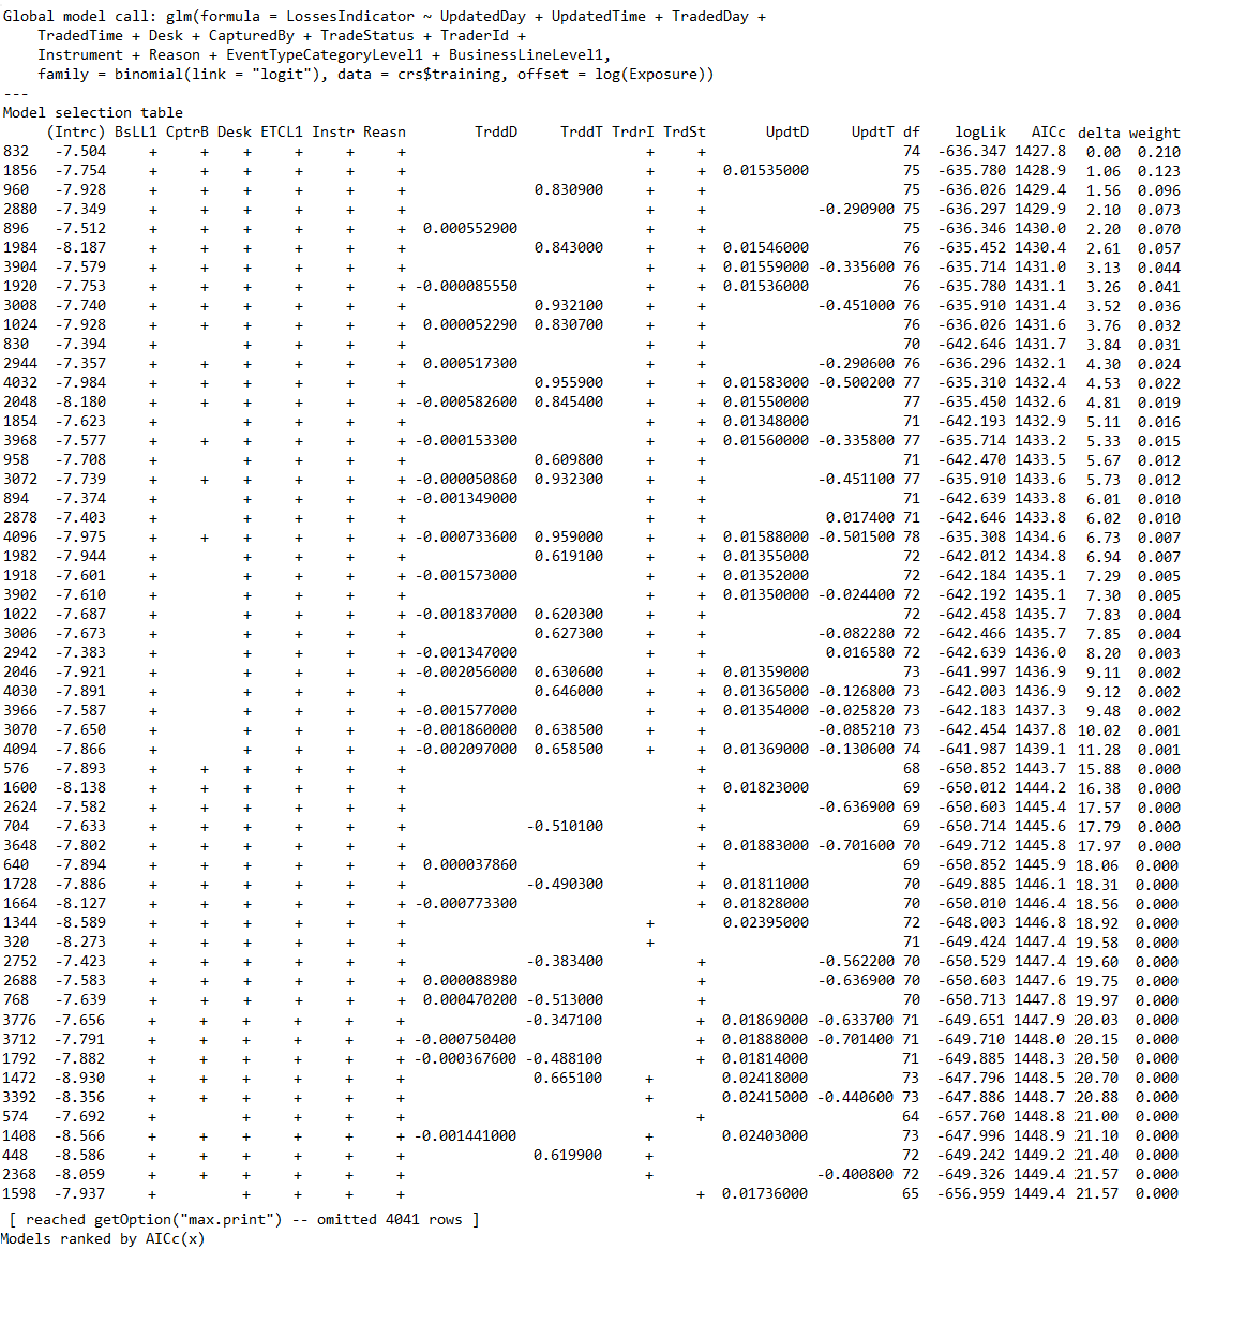
\includegraphics[height=20cm, width=15cm]{Dredge_bin.pdf}
\caption[Data dredging]{Model selection data mining exercise}
\label{Dredge}
\end{figure}

\subsection{We use \texttt{get.models} function to generate a list in which its objects are the fitted models. We will also use the "model.avg" function to do a model averaging based on AICc.}
\label{sec:Model averaging function}

\small

\begin{Shaded}
\begin{Highlighting}[]
\NormalTok{cl <-}\StringTok{ }\KeywordTok{makeCluster}\NormalTok{(}\DecValTok{2}\NormalTok{) }\CommentTok{# Assign R cores to the job }
\NormalTok{Amodel <-}\StringTok{ }\KeywordTok{model.avg}\NormalTok{(}\KeywordTok{get.models}\NormalTok{(freqfits, }\DataTypeTok{subset =} \OtherTok{TRUE}\NormalTok{))}
\KeywordTok{summary}\NormalTok{(Amodel)}
\KeywordTok{stopCluster}\NormalTok{(cl) }
\end{Highlighting}
\end{Shaded}

\normalsize

Now we have AICc values for our models and we have the average model (or
mean model).

\begin{figure}
\centering
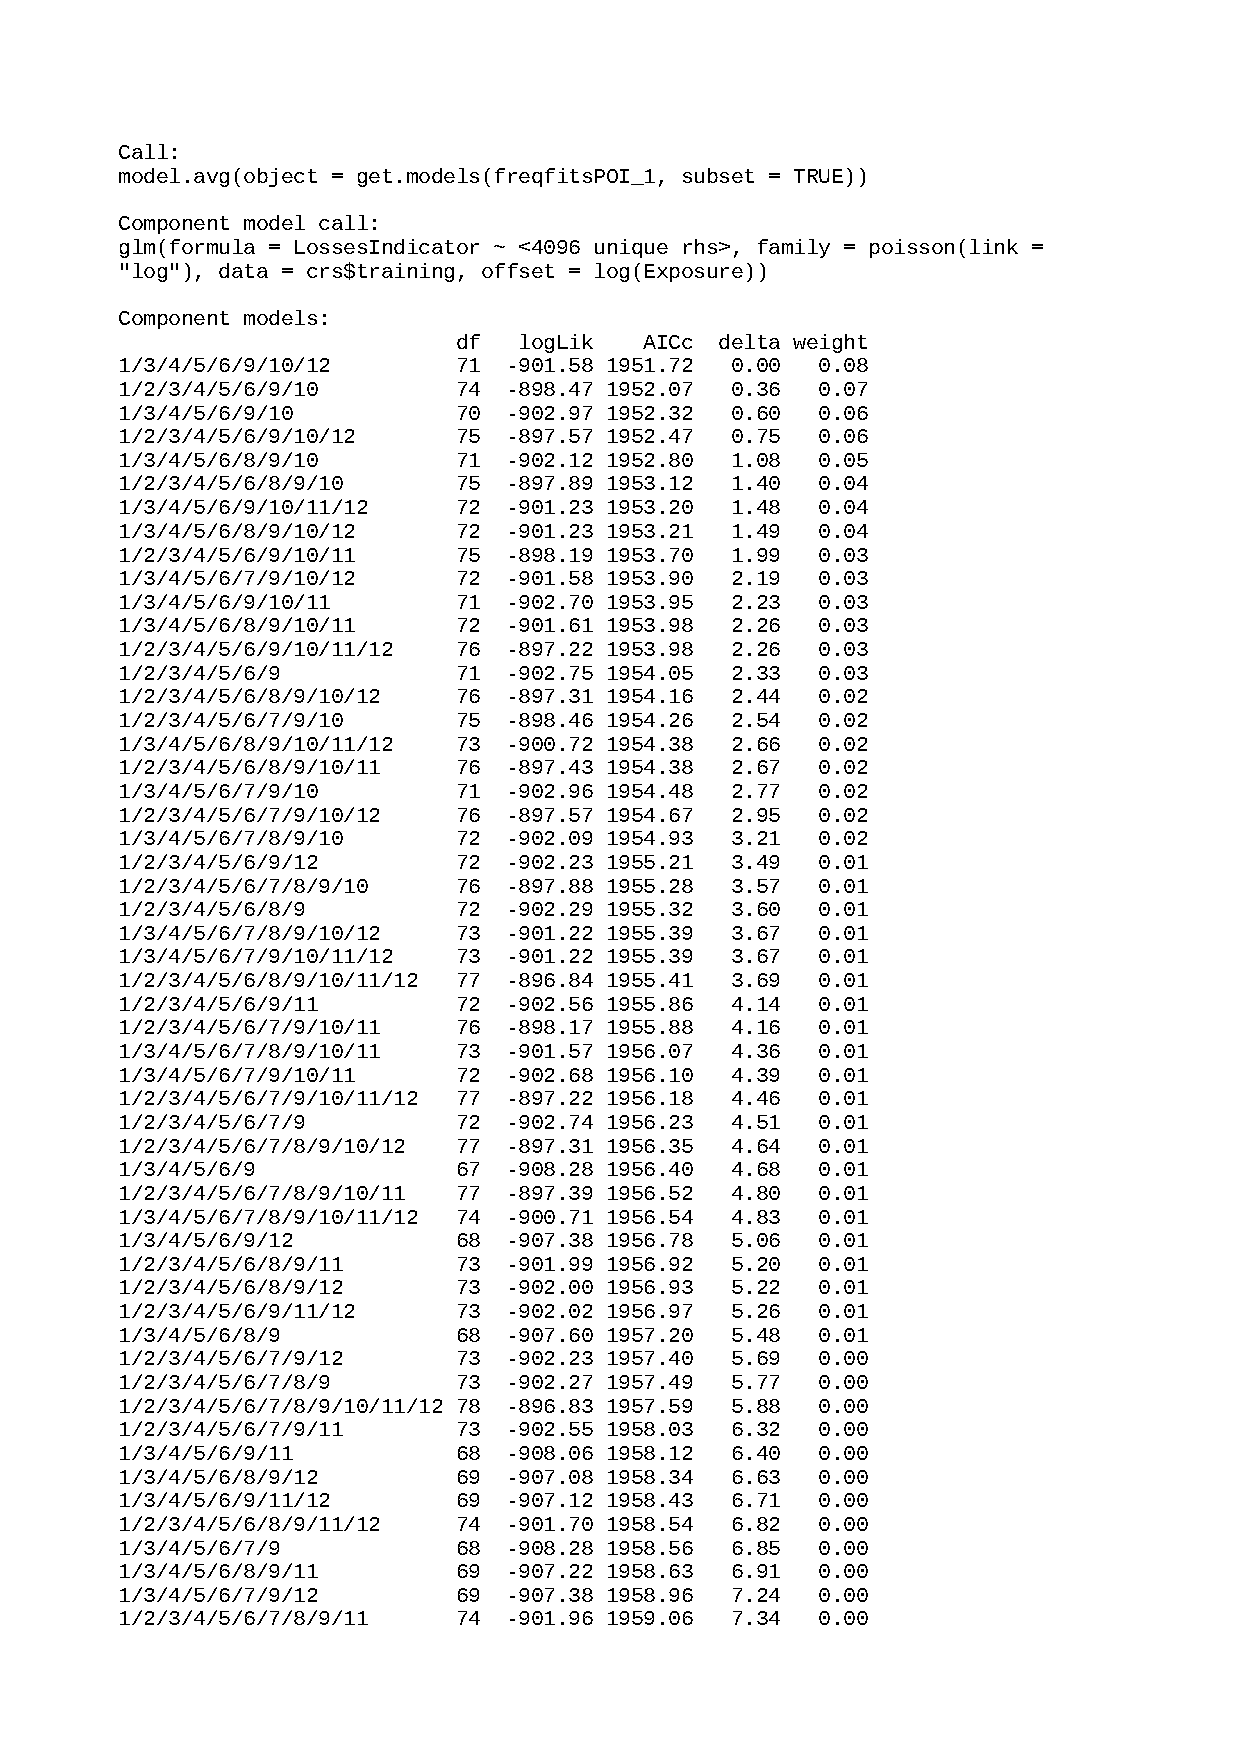
\includegraphics[scale=1.0]{Average_model_Training_1.pdf}
\caption[]{Estimation of some Poisson distribution for target variable \texttt{LossesIndicator} showing the 4096 component models and their respective AICc values for our models giving rise to the average (mean) model \texttt{Amodel}}
\label{AModel_Summary1}
\end{figure}

\begin{figure}
\centering
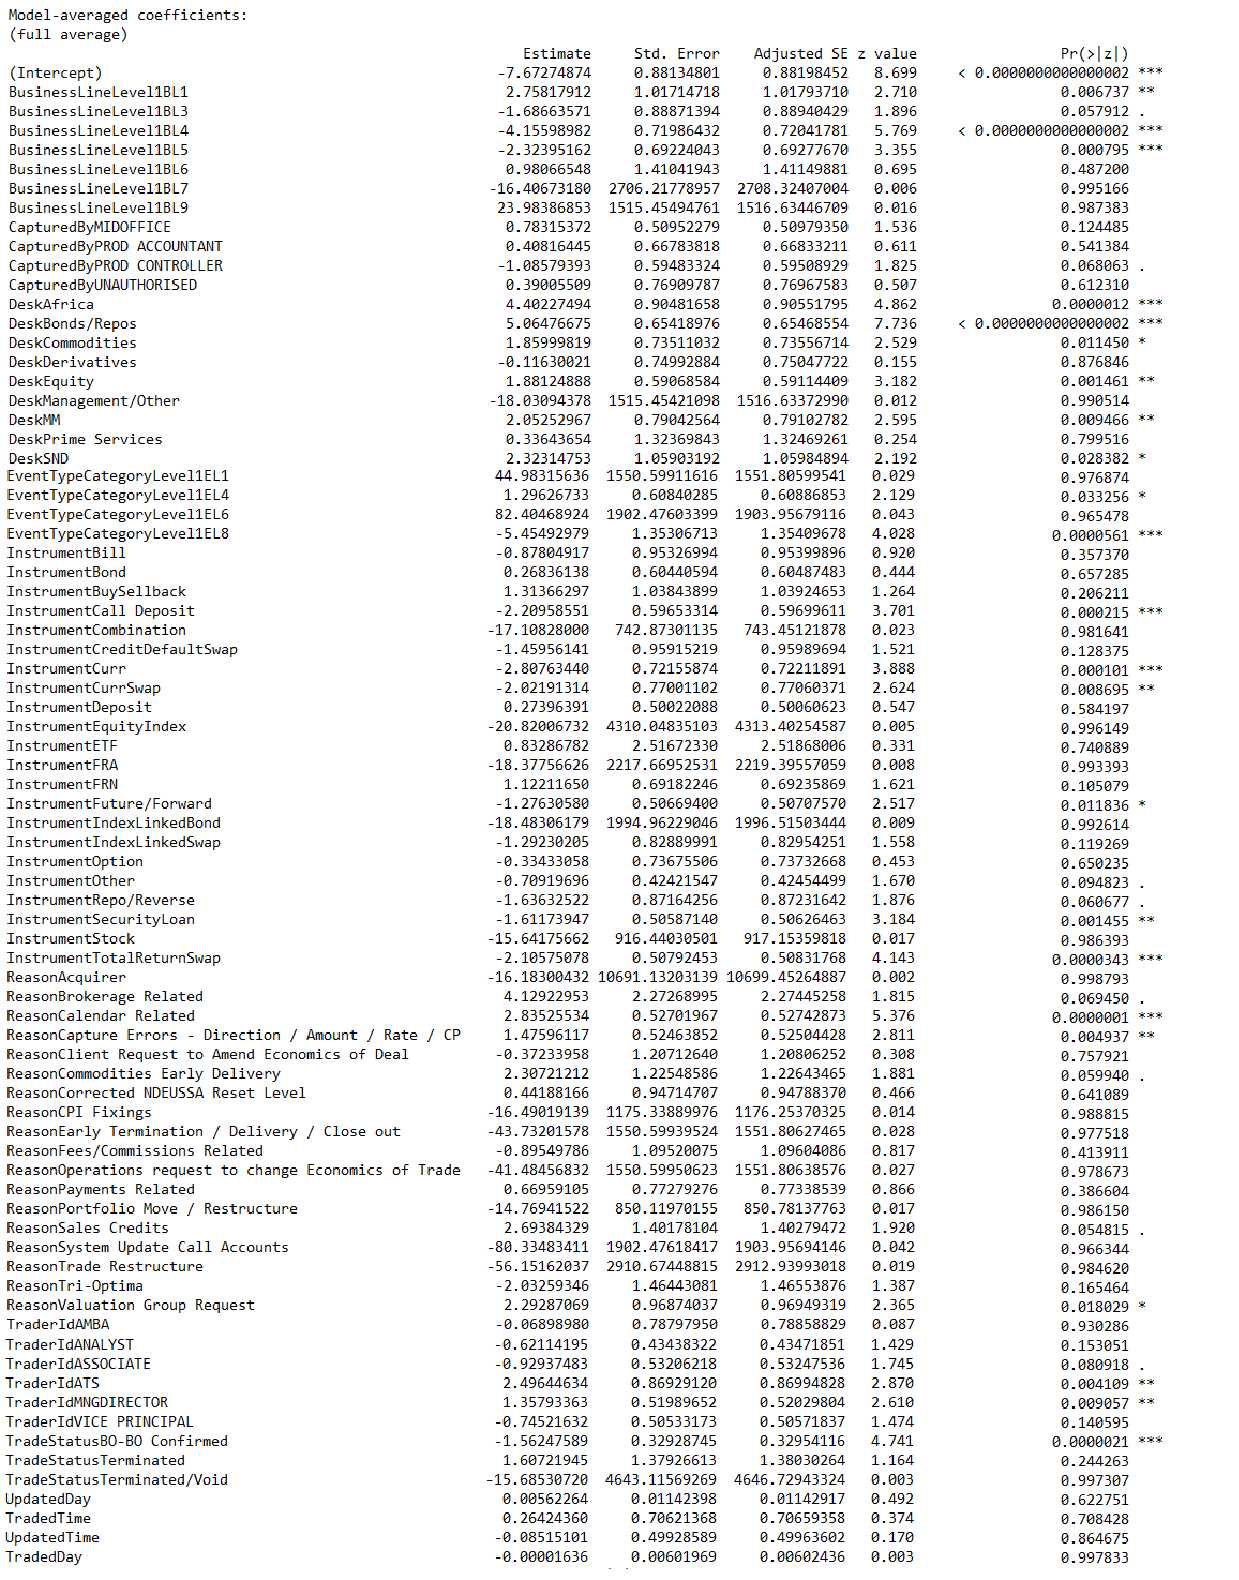
\includegraphics[height=20cm, width=15cm]{Get_models_bin2.pdf}
\caption[Poisson GLM Amodel summary statistics]{Continued from \ref{AModel_Summary1}}
\label{AModel_Summary2}
\end{figure}

\begin{figure}
\centering
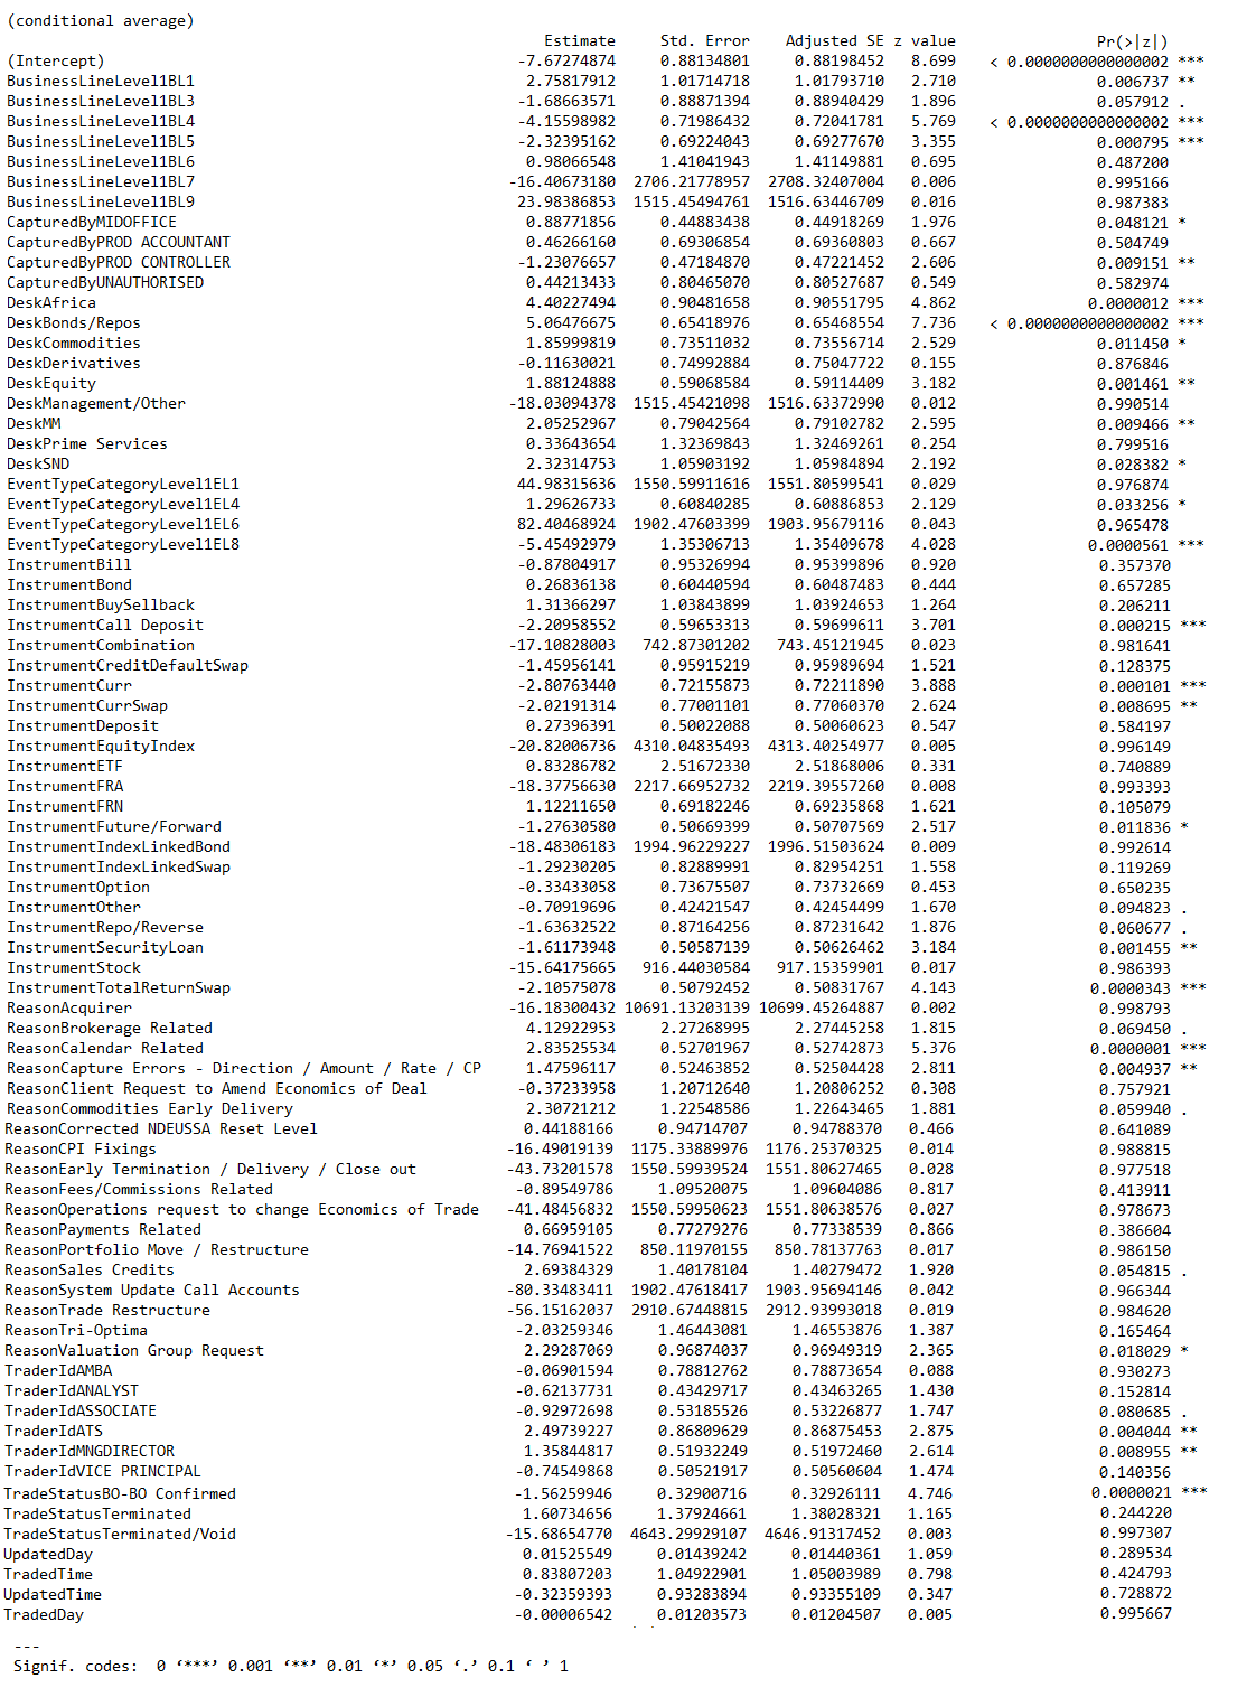
\includegraphics[height=20cm, width=15cm]{Get_models_bin3.pdf}
\caption[Model averaging]{Continued from \ref{AModel_Summary2}}
\label{Poisson GLM Amodel summary statistics continued}
\end{figure}

\subsection{Evaluate model performance on the test dataset}
\label{sec:Evaluate model performance on the test dataset}

Obtain the response from the Linear model.

\small

\begin{Shaded}
\begin{Highlighting}[]
\NormalTok{ Av.PredTT <-}\StringTok{ }\KeywordTok{predict}\NormalTok{(Amodel, crs}\OperatorTok{$}\NormalTok{testing, }\DataTypeTok{type =} \StringTok{"response"}\NormalTok{)}
 
 \CommentTok{# Export into excel}
 
\KeywordTok{HTMLStart}\NormalTok{(); }\KeywordTok{HTML}\NormalTok{(}\KeywordTok{data.frame}\NormalTok{(Av.PredTT)); w <-}\StringTok{ }\KeywordTok{HTMLStop}\NormalTok{()}
\KeywordTok{browseURL}\NormalTok{(w)}
 
\KeywordTok{shell}\NormalTok{(}\KeywordTok{paste}\NormalTok{(}\StringTok{"start excel"}\NormalTok{, w))}
\NormalTok{Est <-}\StringTok{ "file:///C:/Users/Mphekeleli/Documents/R PROJECT/OpRiskPHDGitHub/}
\StringTok{OpRisk_PHD_Thesis/Data/OPriskDataSet_GoF_Amodel_InCode.csv"}
\NormalTok{pred <-}\StringTok{ }\KeywordTok{read.csv}\NormalTok{(Est,}
                   \DataTypeTok{sep=}\StringTok{","}\NormalTok{,}
                   \DataTypeTok{dec=}\StringTok{"."}\NormalTok{,}
                   \DataTypeTok{na.strings=}\KeywordTok{c}\NormalTok{(}\StringTok{"."}\NormalTok{, }\StringTok{"NA"}\NormalTok{, }\StringTok{""}\NormalTok{, }\StringTok{"?"}\NormalTok{),}
                   \DataTypeTok{strip.white=}\OtherTok{TRUE}\NormalTok{, }\DataTypeTok{encoding=}\StringTok{"UTF-8"}\NormalTok{)}
\end{Highlighting}
\end{Shaded}

\normalsize

Generate the confusion matrix showing counts and generate an ROC curve
for the GLM model on the appropriate dataset partition

\begin{Shaded}
\begin{Highlighting}[]
\KeywordTok{confusionMatrix}\NormalTok{(}\KeywordTok{table}\NormalTok{(pred}\OperatorTok{$}\NormalTok{response, crs[[}\StringTok{"testing"}\NormalTok{]][[}\StringTok{"LossesIndicator"}\NormalTok{]]))}

\NormalTok{crs}\OperatorTok{$}\NormalTok{pr <-}\StringTok{ }\NormalTok{Av.PredTT}

\CommentTok{# Remove observations with missing target.}

\NormalTok{no.miss   <-}\StringTok{ }\KeywordTok{na.omit}\NormalTok{(crs[[}\StringTok{"testing"}\NormalTok{]][[}\StringTok{"LossesIndicator"}\NormalTok{]])}
\NormalTok{miss.list <-}\StringTok{ }\KeywordTok{attr}\NormalTok{(no.miss, }\StringTok{"na.action"}\NormalTok{)}
\KeywordTok{attributes}\NormalTok{(no.miss) <-}\StringTok{ }\OtherTok{NULL}

\ControlFlowTok{if}\NormalTok{ (}\KeywordTok{length}\NormalTok{(miss.list))}
\NormalTok{\{}
\NormalTok{  predic <-}\StringTok{ }\KeywordTok{prediction}\NormalTok{(crs}\OperatorTok{$}\NormalTok{pr[}\OperatorTok{-}\NormalTok{miss.list], no.miss)}
\NormalTok{\} }\ControlFlowTok{else}
\NormalTok{\{}
\NormalTok{  predic <-}\StringTok{ }\KeywordTok{prediction}\NormalTok{(crs}\OperatorTok{$}\NormalTok{pr, no.miss)}
\NormalTok{\}}

\NormalTok{pe <-}\StringTok{ }\KeywordTok{performance}\NormalTok{(predic, }\StringTok{"tpr"}\NormalTok{, }\StringTok{"fpr"}\NormalTok{)}
\NormalTok{au <-}\StringTok{ }\KeywordTok{performance}\NormalTok{(predic, }\StringTok{"auc"}\NormalTok{)}\OperatorTok{@}\NormalTok{y.values[[}\DecValTok{1}\NormalTok{]]}
\NormalTok{pd <-}\StringTok{ }\KeywordTok{data.frame}\NormalTok{(}\DataTypeTok{fpr=}\KeywordTok{unlist}\NormalTok{(pe}\OperatorTok{@}\NormalTok{x.values), }\DataTypeTok{tpr=}\KeywordTok{unlist}\NormalTok{(pe}\OperatorTok{@}\NormalTok{y.values))}
\NormalTok{p <-}\StringTok{ }\KeywordTok{ggplot}\NormalTok{(pd, }\KeywordTok{aes}\NormalTok{(}\DataTypeTok{x=}\NormalTok{fpr, }\DataTypeTok{y=}\NormalTok{tpr))}
\NormalTok{p <-}\StringTok{ }\NormalTok{p }\OperatorTok{+}\StringTok{ }\KeywordTok{geom_line}\NormalTok{(}\DataTypeTok{colour=}\StringTok{"red"}\NormalTok{)}
\NormalTok{p <-}\StringTok{ }\NormalTok{p }\OperatorTok{+}\StringTok{ }\KeywordTok{xlab}\NormalTok{(}\StringTok{"False Positive Rate"}\NormalTok{) }\OperatorTok{+}\StringTok{ }\KeywordTok{ylab}\NormalTok{(}\StringTok{"True Positive Rate"}\NormalTok{)}
\NormalTok{p <-}\StringTok{ }\NormalTok{p }\OperatorTok{+}\StringTok{ }\KeywordTok{ggtitle}\NormalTok{(}\StringTok{"ROC Curve Linear OPriskDataSet_exposure.csv [validate] LossesIndicator"}\NormalTok{)}
\NormalTok{p <-}\StringTok{ }\NormalTok{p }\OperatorTok{+}\StringTok{ }\KeywordTok{theme}\NormalTok{(}\DataTypeTok{plot.title=}\KeywordTok{element_text}\NormalTok{(}\DataTypeTok{size=}\DecValTok{10}\NormalTok{))}
\NormalTok{p <-}\StringTok{ }\NormalTok{p }\OperatorTok{+}\StringTok{ }\KeywordTok{geom_line}\NormalTok{(}\DataTypeTok{data=}\KeywordTok{data.frame}\NormalTok{(), }\KeywordTok{aes}\NormalTok{(}\DataTypeTok{x=}\KeywordTok{c}\NormalTok{(}\DecValTok{0}\NormalTok{,}\DecValTok{1}\NormalTok{), }\DataTypeTok{y=}\KeywordTok{c}\NormalTok{(}\DecValTok{0}\NormalTok{,}\DecValTok{1}\NormalTok{)), }\DataTypeTok{colour=}\StringTok{"grey"}\NormalTok{)}
\NormalTok{p <-}\StringTok{ }\NormalTok{p }\OperatorTok{+}\StringTok{ }\KeywordTok{annotate}\NormalTok{(}\StringTok{"text"}\NormalTok{, }\DataTypeTok{x=}\FloatTok{0.50}\NormalTok{, }\DataTypeTok{y=}\FloatTok{0.00}\NormalTok{, }\DataTypeTok{hjust=}\DecValTok{0}\NormalTok{, }\DataTypeTok{vjust=}\DecValTok{0}\NormalTok{, }\DataTypeTok{size=}\DecValTok{5}\NormalTok{,}
                  \DataTypeTok{label=}\KeywordTok{paste}\NormalTok{(}\StringTok{"AUC ="}\NormalTok{, }\KeywordTok{round}\NormalTok{(au, }\DecValTok{2}\NormalTok{)))}
\KeywordTok{print}\NormalTok{(p)}

\CommentTok{# Calculate the area under the curve for the plot.}


\CommentTok{# Remove observations with missing target.}

\NormalTok{no.miss   <-}\StringTok{ }\KeywordTok{na.omit}\NormalTok{(crs[[}\StringTok{"testing"}\NormalTok{]][[}\StringTok{"LossesIndicator"}\NormalTok{]])}
\NormalTok{miss.list <-}\StringTok{ }\KeywordTok{attr}\NormalTok{(no.miss, }\StringTok{"na.action"}\NormalTok{)}
\KeywordTok{attributes}\NormalTok{(no.miss) <-}\StringTok{ }\OtherTok{NULL}

\ControlFlowTok{if}\NormalTok{ (}\KeywordTok{length}\NormalTok{(miss.list))}
\NormalTok{\{}
\NormalTok{  predic <-}\StringTok{ }\KeywordTok{prediction}\NormalTok{(crs}\OperatorTok{$}\NormalTok{pr[}\OperatorTok{-}\NormalTok{miss.list], no.miss)}
\NormalTok{\} }\ControlFlowTok{else}
\NormalTok{\{}
\NormalTok{  predic <-}\StringTok{ }\KeywordTok{prediction}\NormalTok{(crs}\OperatorTok{$}\NormalTok{pr, no.miss)}
\NormalTok{\}}
\KeywordTok{performance}\NormalTok{(predic, }\StringTok{"auc"}\NormalTok{)}
\end{Highlighting}
\end{Shaded}

\begin{figure}
\centering
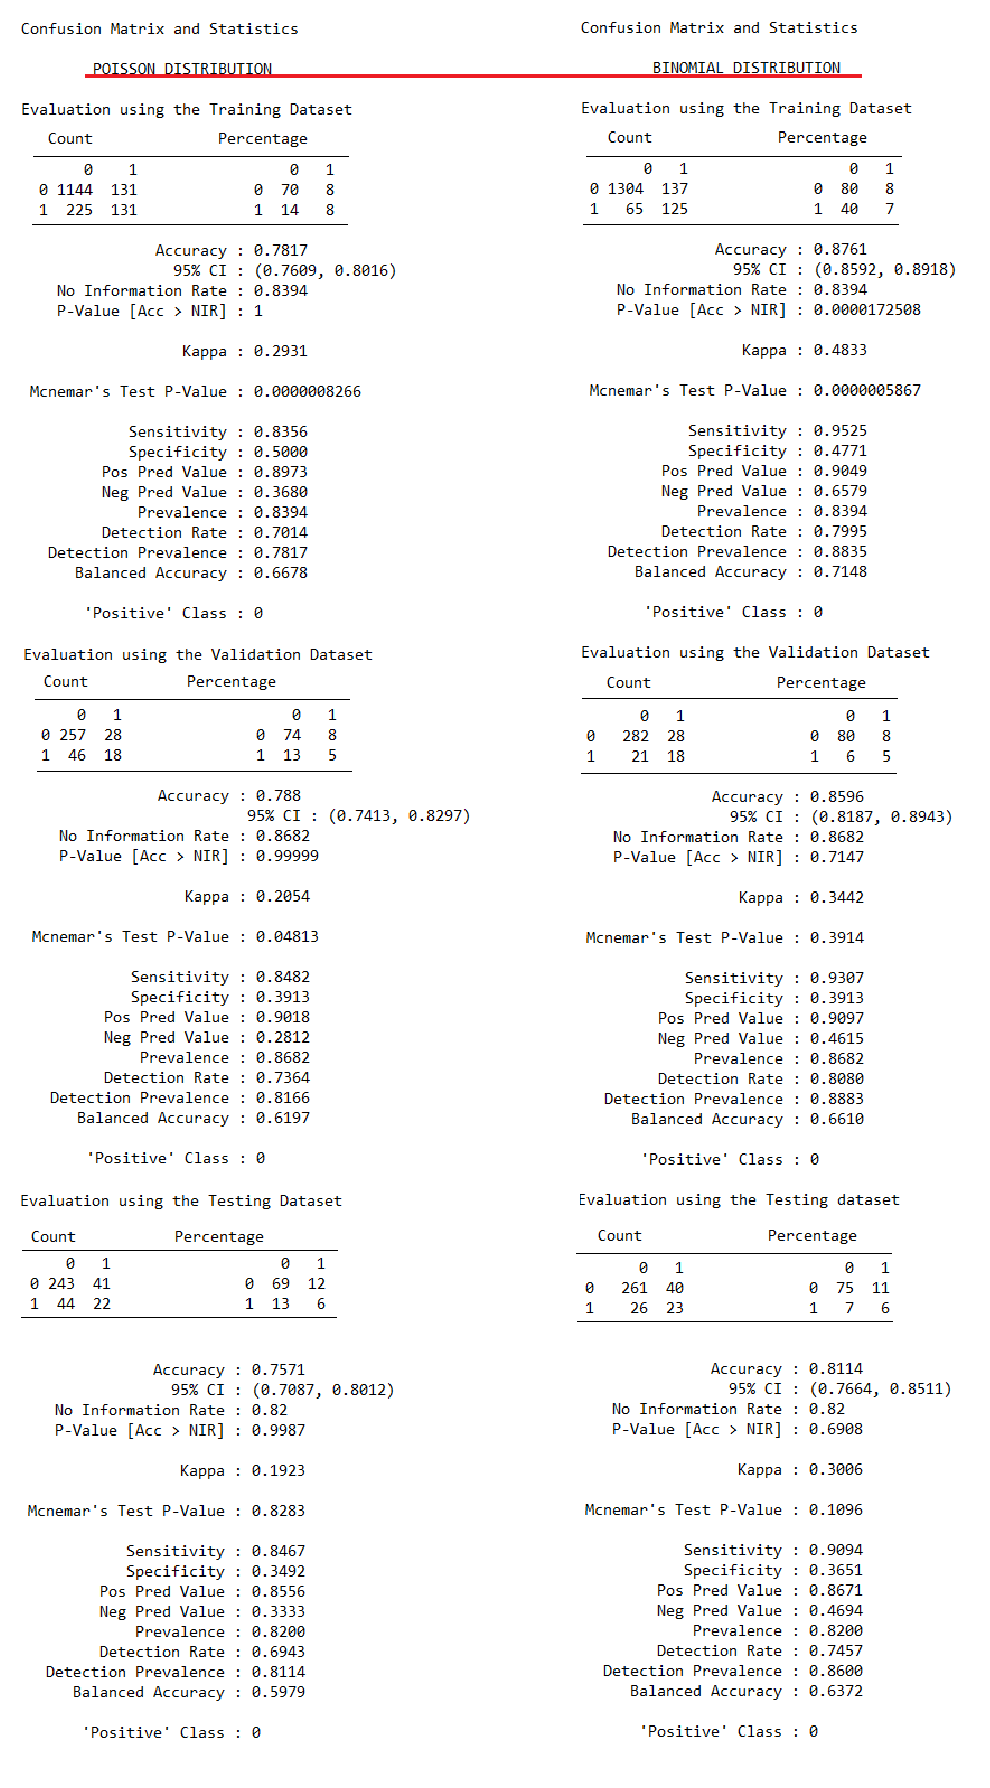
\includegraphics[height=20cm, width=15cm]{ConfusionMatrix_Appendix.eps}
\caption[Confusion Matrices comparison]{Comparison of Poisson, Binomial GLM's confusion matrices for Training, Validation \& Testing datasets}
\label{ConfusionMatrixAll}
\end{figure}

\begin{figure}[t!] % "[t!]" placement specifier just for this example
\begin{subfigure}{0.48\textwidth}
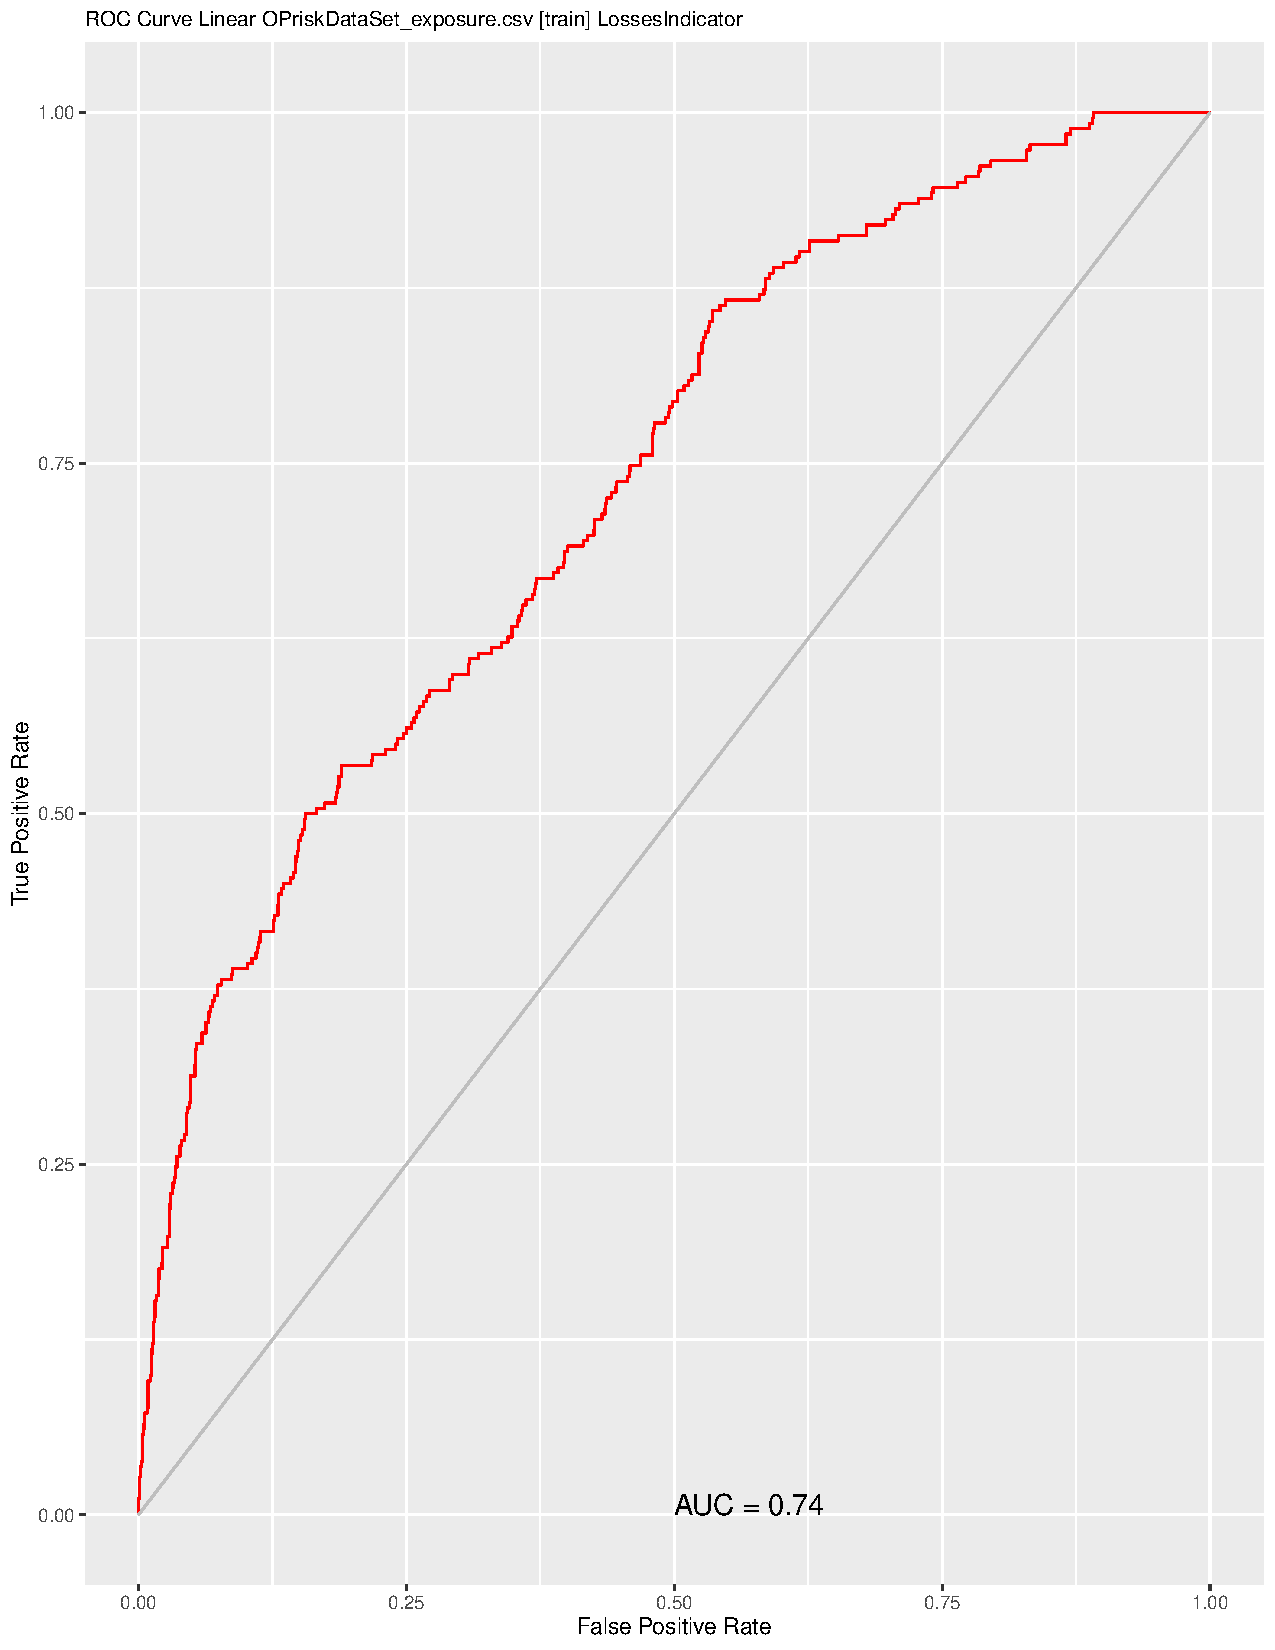
\includegraphics[width=\linewidth]{POI_ROC_Training.pdf}
\caption{AUC for poisson parameter depicting model's performance on the training set} \label{POI_ROC_Train}
\end{subfigure}\hspace*{\fill}
\begin{subfigure}{0.48\textwidth}
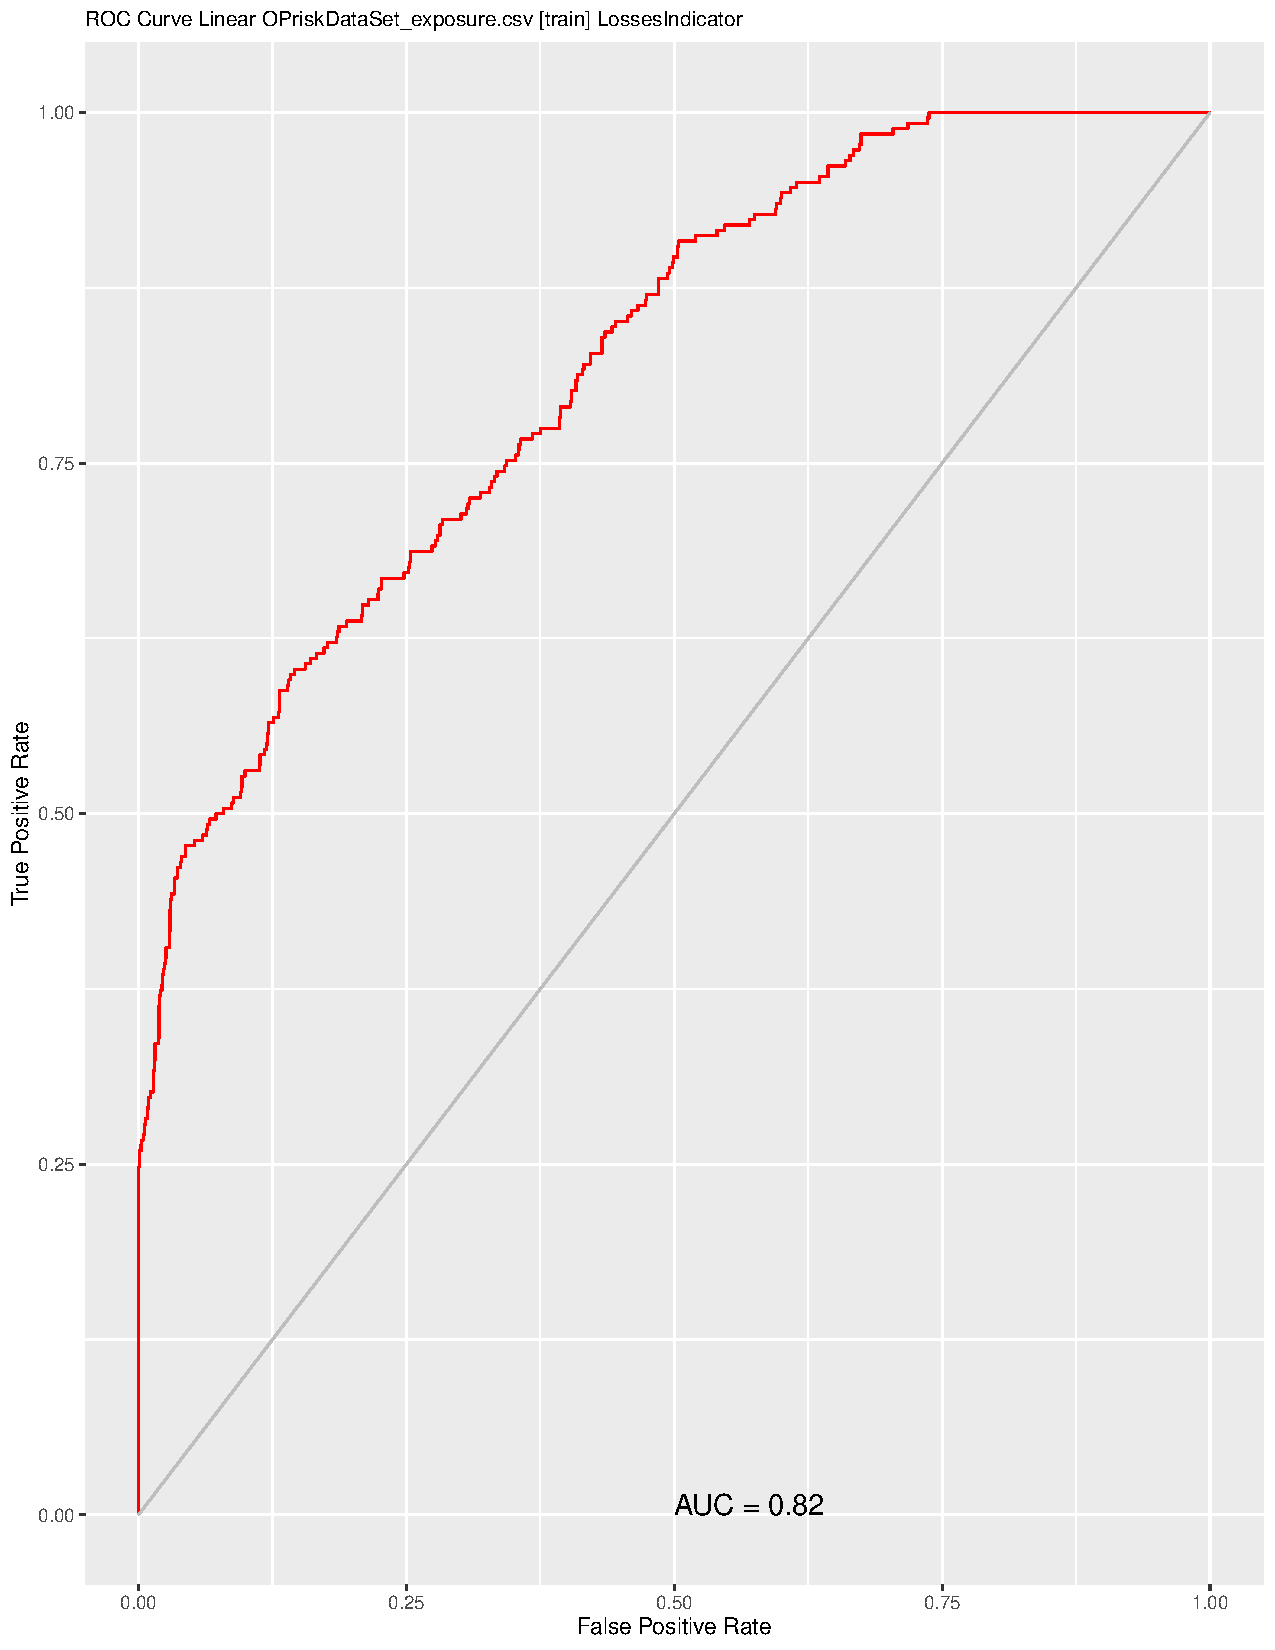
\includegraphics[width=\linewidth]{BIN_ROC_Training.pdf}
\caption{AUC for binomial parameters depicting model's performance on the training set} \label{BIN_ROC_Train}
\end{subfigure}

\medskip
\begin{subfigure}{0.48\textwidth}
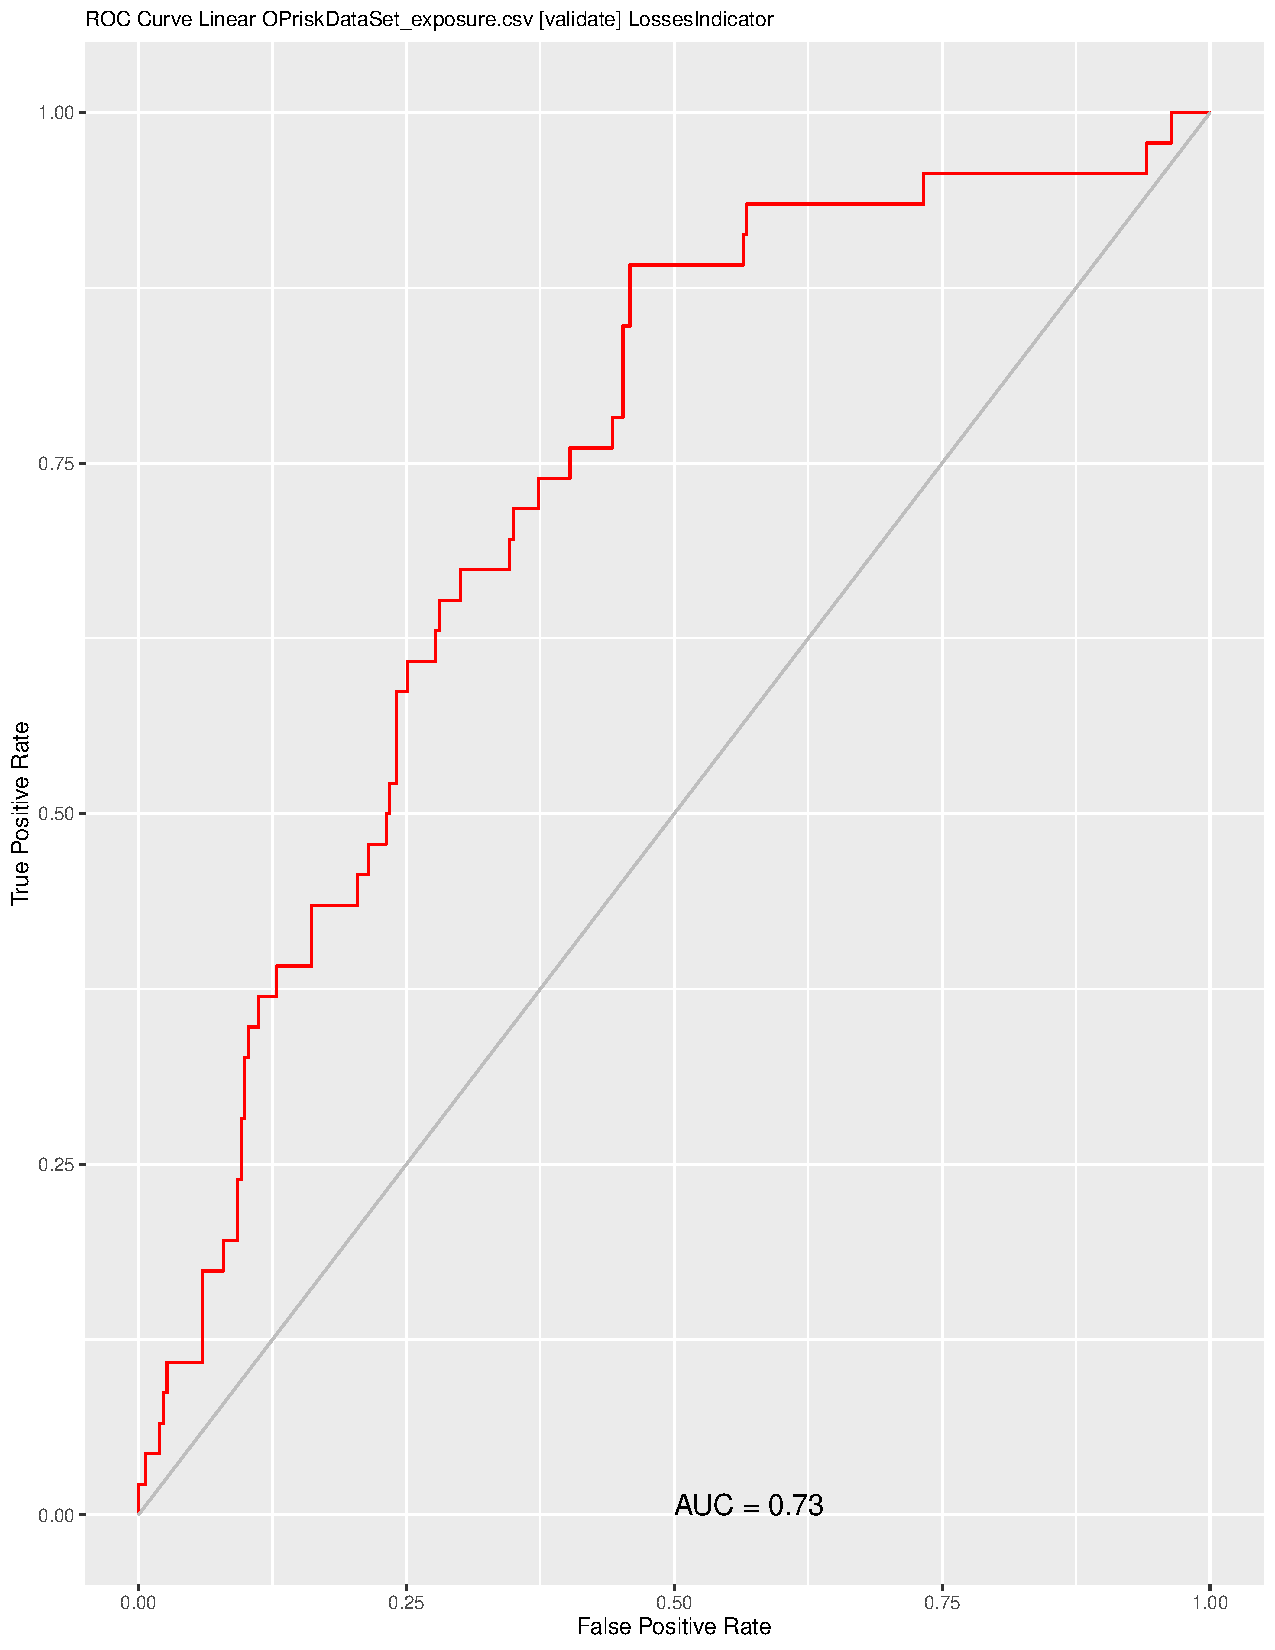
\includegraphics[width=\linewidth]{POI_ROC_Validation.pdf}
\caption{As in (a) but depicting model's performance on the validation set} \label{POI_ROC_Validate}
\end{subfigure}\hspace*{\fill}
\begin{subfigure}{0.48\textwidth}
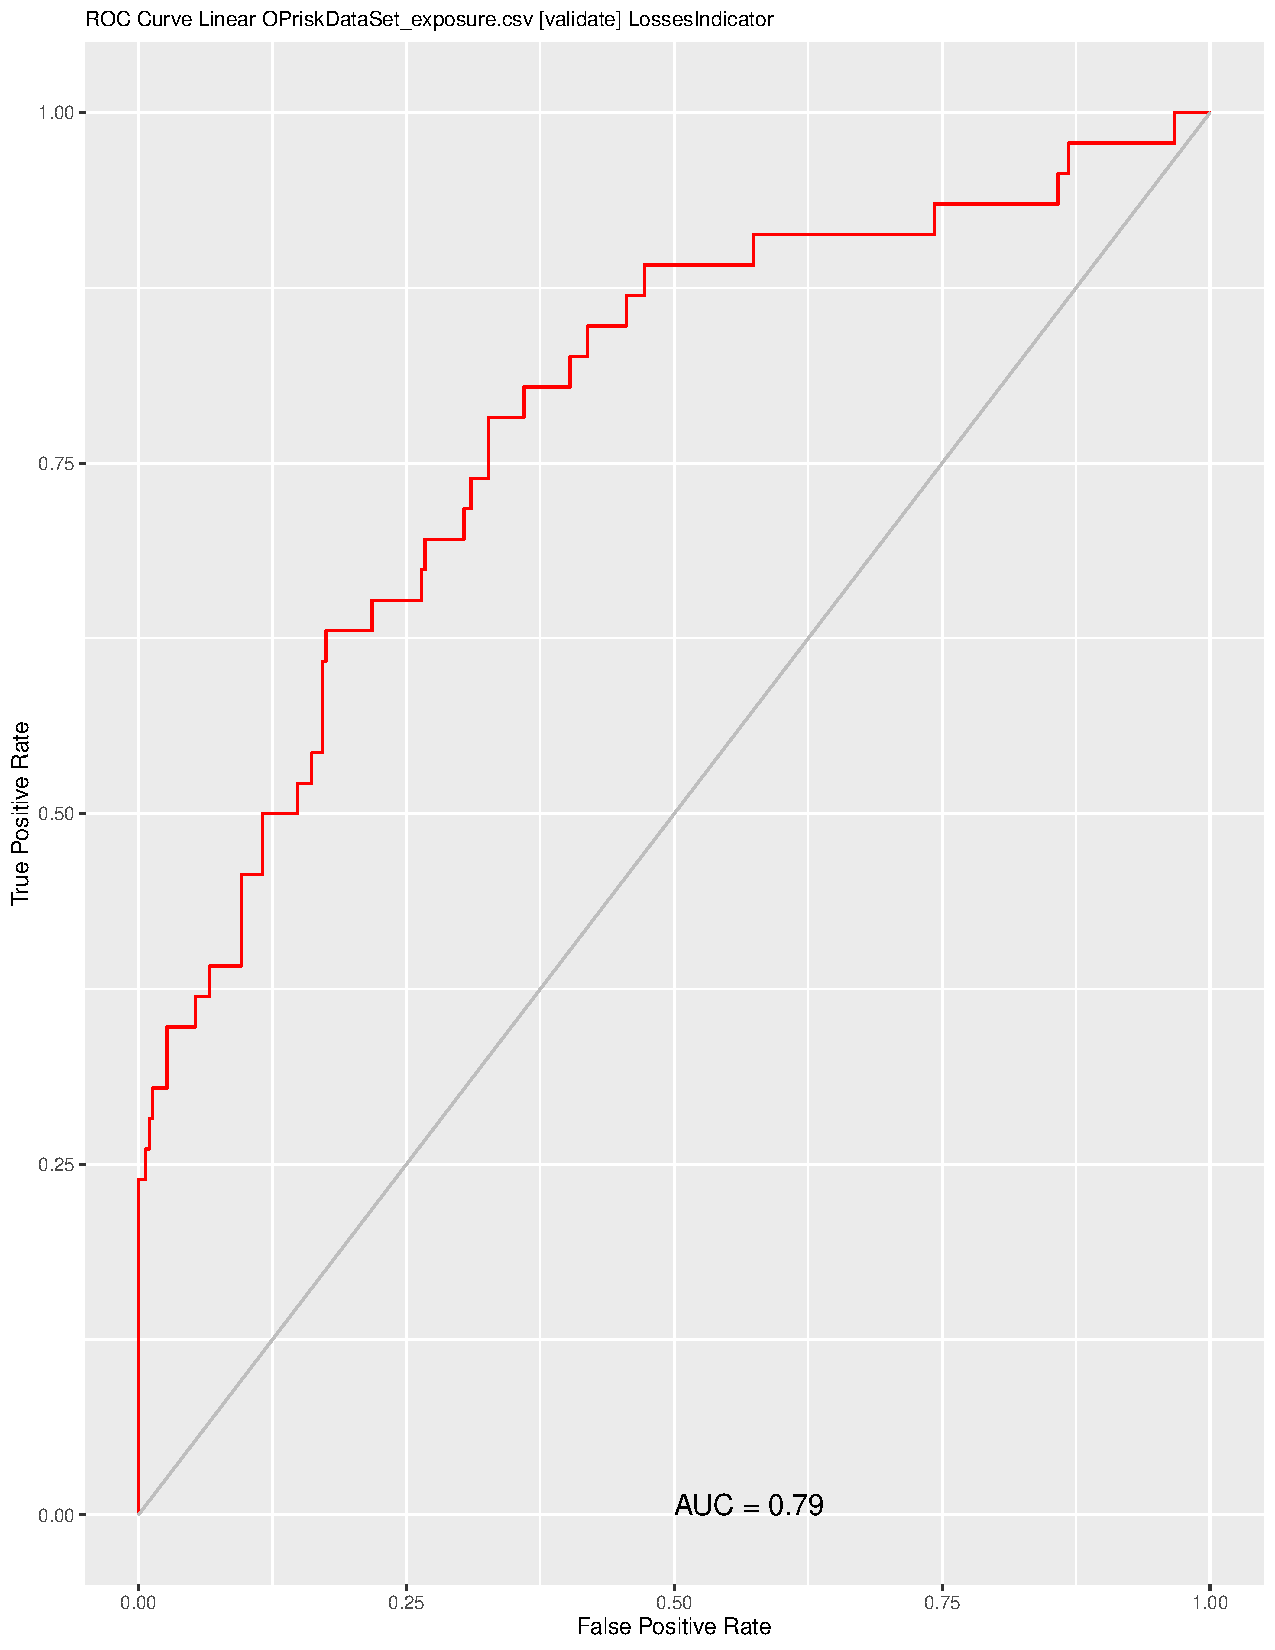
\includegraphics[width=\linewidth]{BIN_ROC_Validation.pdf}
\caption{As in (b) but depicting model's performance on the validation set} \label{BIN_ROC_Validate}
\end{subfigure}

\medskip
\begin{subfigure}{0.48\textwidth}
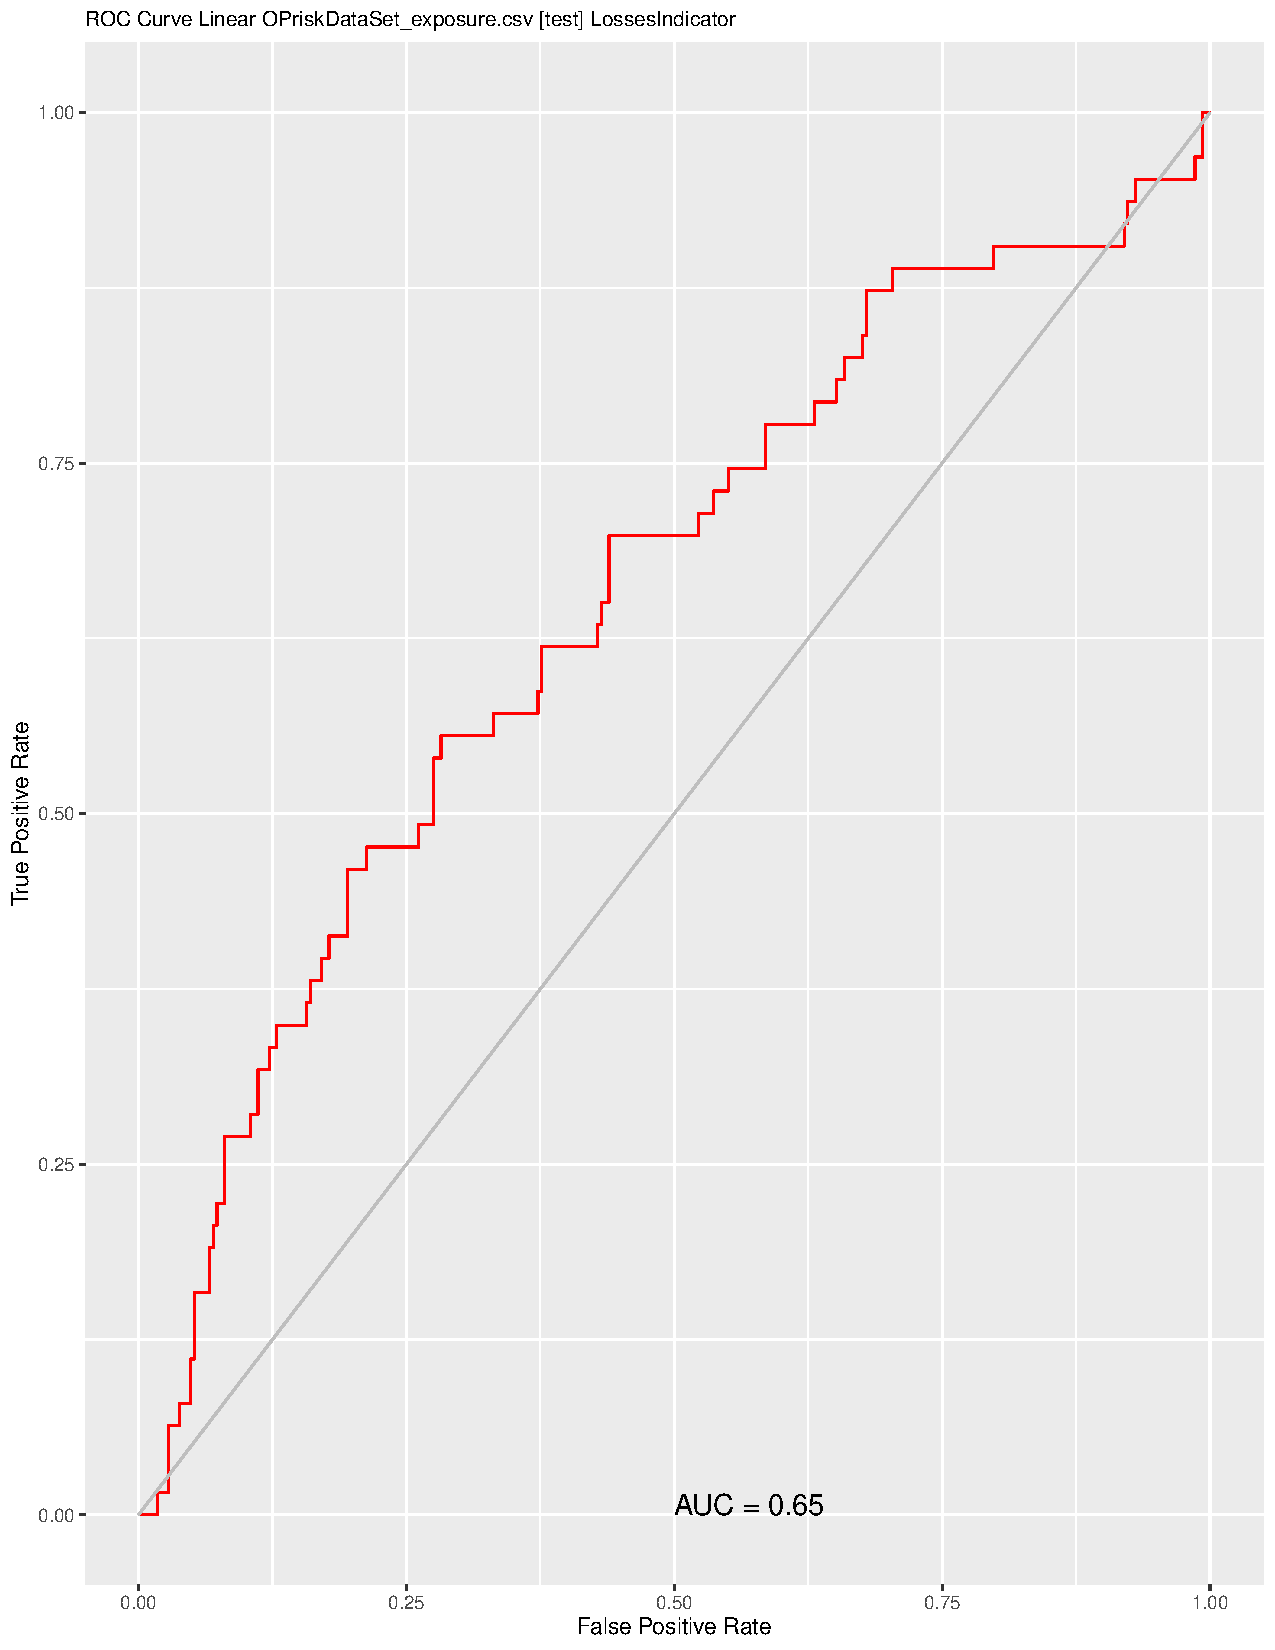
\includegraphics[width=\linewidth]{POI_ROC_Testing.pdf}
\caption{As in (a) \& (c) depicting model's performance on the testing set} \label{POI_ROC_Test}
\end{subfigure}\hspace*{\fill}
\begin{subfigure}{0.48\textwidth}
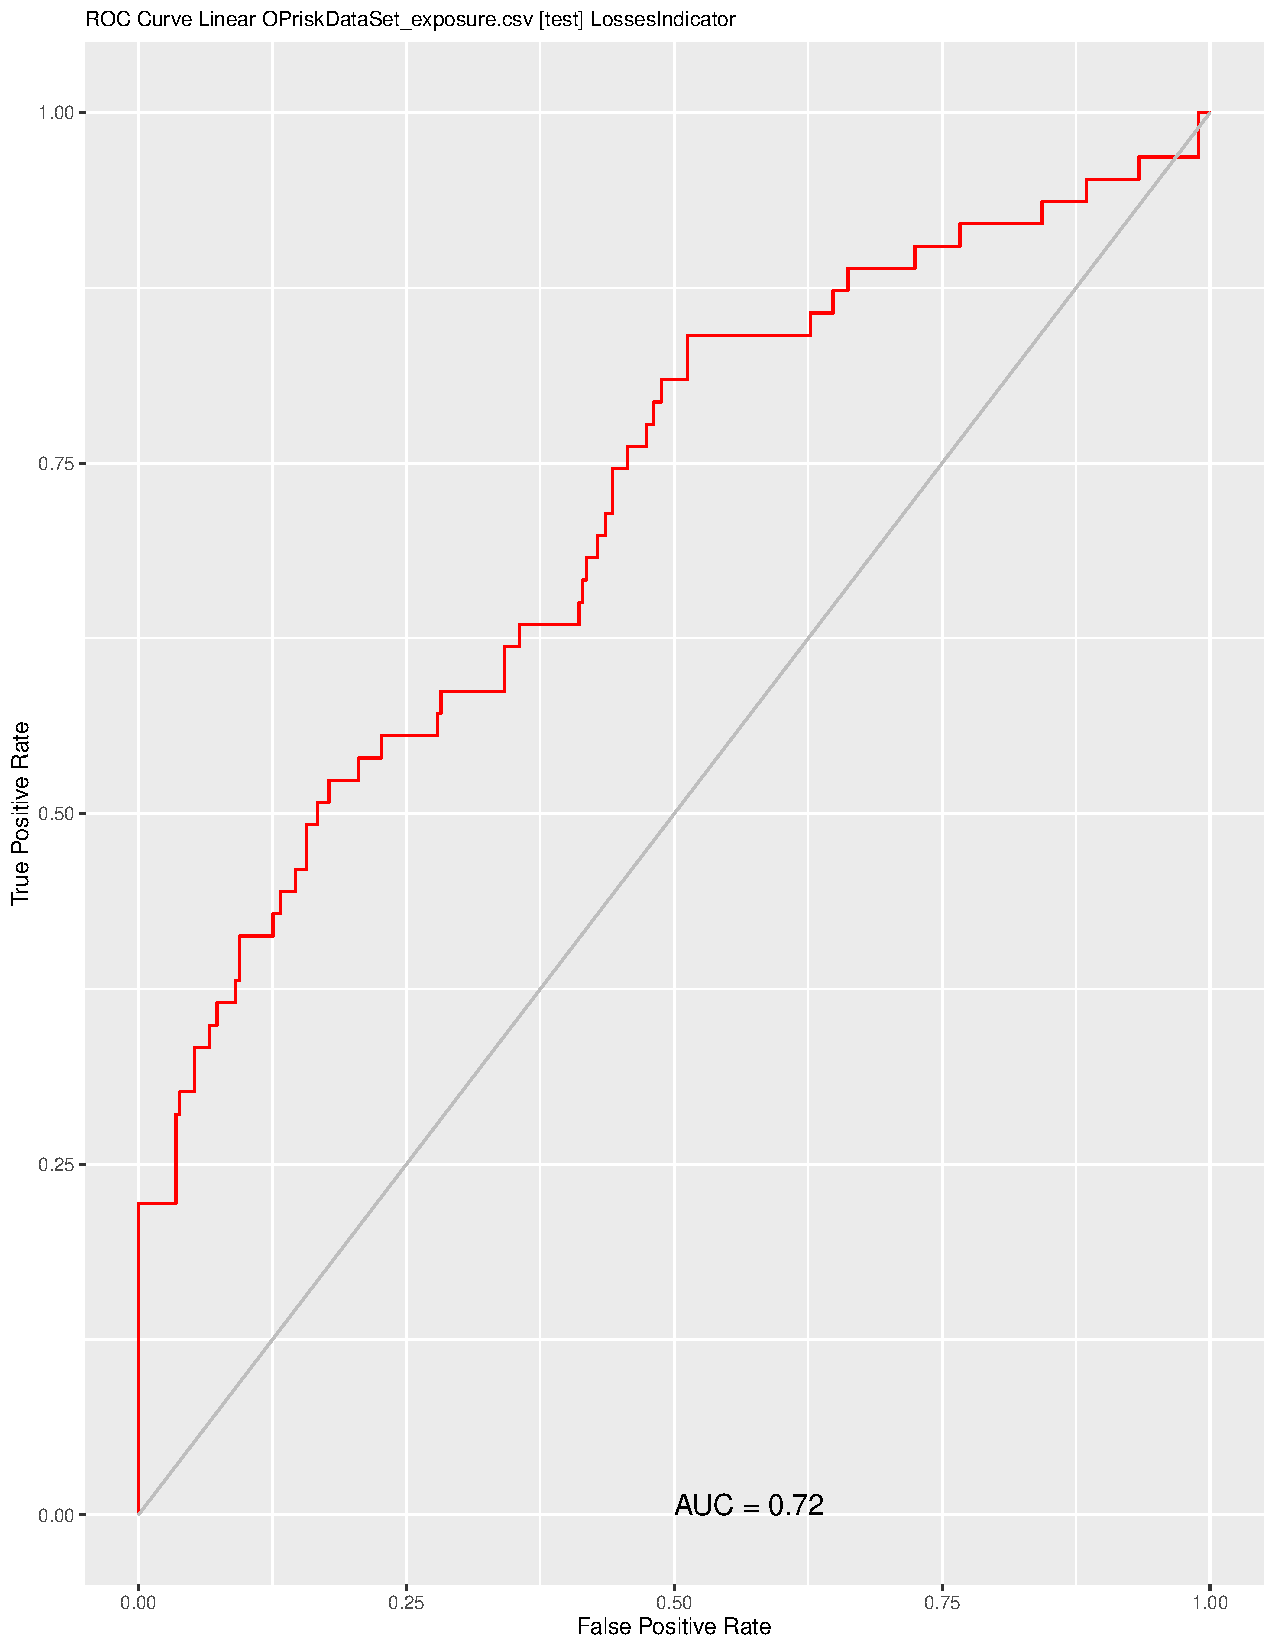
\includegraphics[width=\linewidth]{BIN_ROC_Testing.pdf}
\caption{As in (b) \& (d) depicting model's performance on the testing set} \label{BIN_ROC_Test}
\end{subfigure}

\caption{Comparison of area under the curve (AUC) for the Poisson, Binomial GLM ROC curve for training, validation and testing datasets} \label{ROCCurveAll}
\end{figure}

\clearpage

\section{Data augmentation code: Extrapolation simulation in Matlab}
\label{sec:Data augmentation code: Extrapolation simulation in Matlab}

Notably, the code for the predict condition was run via the Matlab
Terminal:

\small

\begin{Shaded}
\begin{Highlighting}[]

\ExtensionTok\NormalTok{ generate the vector DD}

\ExtensionTok{DDD}\NormalTok{ = 1:31}\KeywordTok{;}

\ExtensionTok\NormalTok{ generate the vector UUU}

\ExtensionTok{UUU}\NormalTok{ = 2013 : -1 : 2006}\KeywordTok{;}

\ExtensionTok\NormalTok{ Years}
\ExtensionTok{Thirty_five_days}\NormalTok{ = [UUU}\StringTok{';UUU'}\KeywordTok{;}\ExtensionTok{UUU}\StringTok{';UUU(1:end-1)'}\NormalTok{]}\KeywordTok{;}
\ExtensionTok{%Months}
\ExtensionTok{Thirty_five_days2}\NormalTok{ = [VVV}\StringTok{';VVV'}\KeywordTok{;}\ExtensionTok{VVV}\NormalTok{(1:7)}\StringTok{'];}
\StringTok\NormalTok{ The updated time algorithm}

\ExtensionTok{%}\NormalTok{ initializing the time matrix}
\KeywordTok{for} \ExtensionTok{i}\NormalTok{ = 1 : length(UUU)}
    
    \ExtensionTok{UUU_trans}\DataTypeTok{\{i\}}\NormalTok{ = num2cell(zeros(1,12));}
    
\ExtensionTok{end}

\KeywordTok{for} \ExtensionTok{i}\NormalTok{ = 1 : length(UUU)}
    \KeywordTok{for} \ExtensionTok{j}\NormalTok{ = 1 : length(UUU_trans}\DataTypeTok{\{1,1\}}\NormalTok{)}
        
        \ExtensionTok{UUU_TRANS}\DataTypeTok{\{1,i\}\{1,j\}}\NormalTok{ = num2cell(zeros(31,4));}
    \ExtensionTok{end}
    
\ExtensionTok{end}

\ExtensionTok\NormalTok{ filling in the time matrix}
\KeywordTok{for} \ExtensionTok{i}\NormalTok{ = 1 : length(UUU)}
    \KeywordTok{for} \ExtensionTok{j}\NormalTok{ = 1 : length(UUU_trans}\DataTypeTok{\{1,1\}}\NormalTok{)}
        
        \ExtensionTok{UUU_TRANS}\DataTypeTok{\{1,i\}\{1,j\}}\NormalTok{(:,end) = }\ExtensionTok{num2cell}\NormalTok{((1:31)}\StringTok{');}
\StringTok{        UUU_TRANS\{1,i\}\{1,j\}(:,end-1) = num2cell(VVV(j));}
\StringTok{        }
\StringTok{        }
\StringTok{        }
\StringTok{    end}
\StringTok{    }
\StringTok{end}

\StringTok{UUU = num2cell(UUU);}
\StringTok{%         UUU = sortrows(UUU,2);}


\StringTok{for i = 1 : length(UUU)}
\StringTok{    for j = 1 : length(UUU_trans\{1,1\})}
\StringTok{        for k = 1 : length(UUU_TRANS\{1,5\}\{1,1\})}
\StringTok{            % PART 1}
\StringTok{            UUU\{i,j\} =num2cell((((i)^(0)).*((j)^(0)).*rand(1,31)));}
\StringTok{            UUU\{i,j\} = UUU\{i,j\}'}\NormalTok{;}
            \ExtensionTok{UUU}\DataTypeTok{\{i,j\}}\NormalTok{(:,2) = }\ExtensionTok{num2cell}\NormalTok{(Thirty_five_days(:,1));}
            \ExtensionTok{UUU}\DataTypeTok{\{i,j\}}\NormalTok{ = sortrows(UUU}\DataTypeTok{\{i,j\}}\NormalTok{,1);}
            
            \ExtensionTok{%PART}\NormalTok{ 2}
            \ExtensionTok{UUU2}\DataTypeTok{\{i,j\}}\NormalTok{ =num2cell((((i)^}\KeywordTok{(}\ExtensionTok{0}\KeywordTok{)}\NormalTok{)}\ExtensionTok{.*}\NormalTok{((j)^}\KeywordTok{(}\ExtensionTok{0}\KeywordTok{)}\NormalTok{)}\ExtensionTok{.*rand}\NormalTok{(1,31)));}
            \ExtensionTok{UUU2}\DataTypeTok{\{i,j\}}\NormalTok{ = UUU2}\DataTypeTok{\{i,j\}}\StringTok{';}
\StringTok{            UUU2\{i,j\}(:,2) = num2cell(Thirty_five_days2(:,1));}
\StringTok{            UUU2\{i,j\} = sortrows(UUU2\{i,j\},1);}
\StringTok{            % PART 3}
\StringTok{            UUU3\{i,j\} =num2cell((((i)^(0)).*((j)^(0)).*rand(1,31)));}
\StringTok{            UUU3\{i,j\} = UUU3\{i,j\}'}\KeywordTok{;}
            \ExtensionTok{UUU3}\DataTypeTok{\{i,j\}}\NormalTok{(:,2) = }\ExtensionTok{num2cell}\NormalTok{(Thirty_five_days3(:,1));}
            \ExtensionTok{UUU3}\DataTypeTok{\{i,j\}}\NormalTok{ = sortrows(UUU3}\DataTypeTok{\{i,j\}}\NormalTok{,1);}
            \ExtensionTok\NormalTok{ PART 2}
            \ExtensionTok{UUU_TRANS}\DataTypeTok{\{1,i\}\{1,j\}}\NormalTok{(k,end-2) = }\ExtensionTok{UUU2}\DataTypeTok{\{i,j\}}\NormalTok{(k,2);}
            \ExtensionTok{%PART3}
            \ExtensionTok{UUU_TRANS}\DataTypeTok{\{1,i\}\{1,j\}}\NormalTok{(k,end-1) = }\ExtensionTok{UUU3}\DataTypeTok{\{i,j\}}\NormalTok{(k,2);}
            \ExtensionTok{rH}\DataTypeTok{\{i,j\}}\NormalTok{ = num2cell(((i)^}\KeywordTok{(}\ExtensionTok{0}\KeywordTok{)}\ExtensionTok{.*}\NormalTok{(j)^}\KeywordTok{(}\ExtensionTok{0}\KeywordTok{)}\NormalTok{)}\ExtensionTok{.*rand}\NormalTok{(H,1));}
            \ExtensionTok{yH}\DataTypeTok{\{i,j\}}\NormalTok{ = rH}\DataTypeTok{\{i,j\}}\NormalTok{(cell2mat( rH}\DataTypeTok{\{i,j\}}\NormalTok{) }\OperatorTok{<}\NormalTok{= }\ExtensionTok{UPD}\NormalTok{);}
            \ExtensionTok{gH}\DataTypeTok{\{i,j\}}\NormalTok{ = num2cell(cell2mat( yH}\DataTypeTok{\{i,j\}}\NormalTok{(1:31)));}
            \ExtensionTok{UUU_TRANS}\DataTypeTok{\{1,i\}\{1,j\}}\NormalTok{(k,end) = }\ExtensionTok{gH}\DataTypeTok{\{i,j\}}\NormalTok{(k,1);}
        \ExtensionTok{end}
    \ExtensionTok{end}
    
\ExtensionTok{end}

\ExtensionTok{UPDATED_TIME}\NormalTok{ = UUU_TRANS}\KeywordTok{;}


\ExtensionTok\NormalTok{ Traded time}

\ExtensionTok\NormalTok{ generate the vector VVV}

\ExtensionTok{VVVT}\NormalTok{ = 1:12}\KeywordTok{;}

\ExtensionTok\NormalTok{ making the full thrity five days vector}
\ExtensionTok{%}\NormalTok{ Years}
\ExtensionTok{Thirty_five_daysT}\NormalTok{ = [UUUT}\StringTok{';UUUT'}\KeywordTok{;}\ExtensionTok{UUUT}\StringTok{';UUUT(1:end-1)'}\NormalTok{]}\KeywordTok{;}
\ExtensionTok{%Months}
\ExtensionTok{Thirty_five_days2T}\NormalTok{ = [VVVT}\StringTok{';VVVT'}\KeywordTok{;}\ExtensionTok{VVVT}\NormalTok{(1:7)}\StringTok{'];}
\StringTok\NormalTok{ The updated time algorithm}

\ExtensionTok{%}\NormalTok{ initializing the time matrix}
\KeywordTok{for} \ExtensionTok{i}\NormalTok{ = 1 : length(UUUT)}
    
    \ExtensionTok{UUU_transT}\DataTypeTok{\{i\}}\NormalTok{ = num2cell(zeros(1,12));}
    
\ExtensionTok{end}

\KeywordTok{for} \ExtensionTok{i}\NormalTok{ = 1 : length(UUUT)}
    \KeywordTok{for} \ExtensionTok{j}\NormalTok{ = 1 : length(UUU_transT}\DataTypeTok{\{1,1\}}\NormalTok{)}
        
        \ExtensionTok{UUU_TRANST}\DataTypeTok{\{1,i\}\{1,j\}}\NormalTok{ = num2cell(zeros(31,4));}
    \ExtensionTok{end}
    
\ExtensionTok{end}

\ExtensionTok\NormalTok{ filling in the time matrix}
\KeywordTok{for} \ExtensionTok{i}\NormalTok{ = 1 : length(UUUT)}
    \KeywordTok{for} \ExtensionTok{j}\NormalTok{ = 1 : length(UUU_transT}\DataTypeTok{\{1,1\}}\NormalTok{)}
        
        \ExtensionTok{UUU_TRANST}\DataTypeTok{\{1,i\}\{1,j\}}\NormalTok{(:,end) = }\ExtensionTok{num2cell}\NormalTok{((1:31)}\StringTok{');}
\StringTok{        UUU_TRANST\{1,i\}\{1,j\}(:,end-1) = num2cell(VVVT(j));}
\StringTok{        }
\StringTok{        }
\StringTok{        }
\StringTok{    end}
\StringTok{    }
\StringTok{end}

\StringTok{UUUT = num2cell(UUUT);}
\StringTok{%         UUU = sortrows(UUU,2);}


\StringTok{for i = 1 : length(UUUT)}
\StringTok{    for j = 1 : length(UUU_transT\{1,1\})}
\StringTok{        for k = 1 : length(UUU_TRANST\{1,5\}\{1,1\})}
\StringTok{            % PART 1}
\StringTok{            UUUT\{i,j\} =num2cell((((i)^(0)).*((j)^(0)).*rand(1,31)));}
\StringTok{            UUUT\{i,j\} = UUUT\{i,j\}'}\NormalTok{;}
            \ExtensionTok{UUUT}\DataTypeTok{\{i,j\}}\NormalTok{(:,2) = }\ExtensionTok{num2cell}\NormalTok{(Thirty_five_daysT(:,1));}
            \ExtensionTok{UUUT}\DataTypeTok{\{i,j\}}\NormalTok{ = sortrows(UUUT}\DataTypeTok{\{i,j\}}\NormalTok{,1);}
            
            \ExtensionTok{%PART}\NormalTok{ 2}
            \ExtensionTok{UUU2T}\DataTypeTok{\{i,j\}}\NormalTok{ =num2cell((((i)^}\KeywordTok{(}\ExtensionTok{0}\KeywordTok{)}\NormalTok{)}\ExtensionTok{.*}\NormalTok{((j)^}\KeywordTok{(}\ExtensionTok{0}\KeywordTok{)}\NormalTok{)}\ExtensionTok{.*rand}\NormalTok{(1,31)));}
            \ExtensionTok{UUU2T}\DataTypeTok{\{i,j\}}\NormalTok{ = UUU2T}\DataTypeTok{\{i,j\}}\StringTok{';}
\StringTok{            UUU2T\{i,j\}(:,2) = num2cell(Thirty_five_days2T(:,1));}
\StringTok{            UUU2T\{i,j\} = sortrows(UUU2T\{i,j\},1);}
\StringTok{            % PART 3}
\StringTok{            UUU3T\{i,j\} =num2cell((((i)^(0)).*((j)^(0)).*rand(1,31)));}
\StringTok{            UUU3T\{i,j\} = UUU3T\{i,j\}'}\KeywordTok{;}
            \ExtensionTok{UUU3T}\DataTypeTok{\{i,j\}}\NormalTok{(:,2) = }\ExtensionTok{num2cell}\NormalTok{(Thirty_five_days3T(:,1));}
            \ExtensionTok{UUU3T}\DataTypeTok{\{i,j\}}\NormalTok{ = sortrows(UUU3T}\DataTypeTok{\{i,j\}}\NormalTok{,1);}
            \ExtensionTok\NormalTok{ PART 2}
            \ExtensionTok{UUU_TRANST}\DataTypeTok{\{1,i\}\{1,j\}}\NormalTok{(k,end-2) = }\ExtensionTok{UUU2T}\DataTypeTok{\{i,j\}}\NormalTok{(k,2);}
            \ExtensionTok{%PART3}
            \ExtensionTok{UUU_TRANST}\DataTypeTok{\{1,i\}\{1,j\}}\NormalTok{(k,end-1) = }\ExtensionTok{UUU3T}\DataTypeTok{\{i,j\}}\NormalTok{(k,2);}
            \ExtensionTok{rHT}\DataTypeTok{\{i,j\}}\NormalTok{ = num2cell(((i)^}\KeywordTok{(}\ExtensionTok{0}\KeywordTok{)}\ExtensionTok{.*}\NormalTok{(j)^}\KeywordTok{(}\ExtensionTok{0}\KeywordTok{)}\NormalTok{)}\ExtensionTok{.*rand}\NormalTok{(HT,1));}
            \ExtensionTok{yHT}\DataTypeTok{\{i,j\}}\NormalTok{ = rHT}\DataTypeTok{\{i,j\}}\NormalTok{(cell2mat( rHT}\DataTypeTok{\{i,j\}}\NormalTok{) }\OperatorTok{<}\NormalTok{= }\ExtensionTok{UPDT}\NormalTok{);}
            \ExtensionTok{gHT}\DataTypeTok{\{i,j\}}\NormalTok{ = num2cell(cell2mat( yHT}\DataTypeTok{\{i,j\}}\NormalTok{(1:31)));}
            \ExtensionTok{UUU_TRANST}\DataTypeTok{\{1,i\}\{1,j\}}\NormalTok{(k,end) = }\ExtensionTok{gHT}\DataTypeTok{\{i,j\}}\NormalTok{(k,1);}
        \ExtensionTok{end}
    \ExtensionTok{end}
    
\ExtensionTok{end}

\ExtensionTok{TRADED_TIME}\NormalTok{ = UUU_TRANST}\KeywordTok{;}

\ExtensionTok\NormalTok{ RULE for correcting the traded time}
\ExtensionTok{SIZZZE}\NormalTok{ = size(UUU_TRANS}\DataTypeTok{\{1,3\}\{1,2\}}\NormalTok{);}
\KeywordTok{for} \ExtensionTok{i}\NormalTok{ = 1 : 8}
    \KeywordTok{for} \ExtensionTok{j}\NormalTok{ = 1 : length(UUU_transT}\DataTypeTok{\{1,1\}}\NormalTok{)}
        \KeywordTok{for} \ExtensionTok{k}\NormalTok{ = 1 : length(UUU_TRANST}\DataTypeTok{\{1,5\}\{1,1\}}\NormalTok{)}
            
            
            \KeywordTok{if}  \ExtensionTok{TRADED_TIME}\DataTypeTok{\{1,i\}\{1,j\}\{k,1\}} \OperatorTok{>}\NormalTok{= UPDATED_TIME}\DataTypeTok{\{1,i\}\{1,j\}\{k,1\}}
                
                \ExtensionTok{TRADED_TIME}\DataTypeTok{\{1,i\}\{1,j\}\{k,1\}}\NormalTok{ = UPDATED_TIME}\DataTypeTok{\{1,i\}\{1,j\}\{k,1\}}\KeywordTok{;}
            \ExtensionTok{end}
                
            \KeywordTok{if} \ExtensionTok{TRADED_TIME}\DataTypeTok{\{1,i\}\{1,j\}\{k,1\}} \OperatorTok{>}\NormalTok{= UPDATED_TIME}\DataTypeTok{\{1,i\}\{1,j\}\{k,1\}}\NormalTok{...}
                    \KeywordTok{&&} \ExtensionTok{TRADED_TIME}\DataTypeTok{\{1,i\}\{1,j\}\{k,2\}} \OperatorTok{>}\NormalTok{= UPDATED_TIME}\DataTypeTok{\{1,i\}\{1,j\}\{k,2\}}
                
                
                \ExtensionTok{TRADED_TIME}\DataTypeTok{\{1,i\}\{1,j\}\{k,1\}}\NormalTok{ = UPDATED_TIME}\DataTypeTok{\{1,i\}\{1,j\}\{k,1\}}\KeywordTok{;}
                \ExtensionTok{TRADED_TIME}\DataTypeTok{\{1,i\}\{1,j\}\{k,2\}}\NormalTok{ = UPDATED_TIME}\DataTypeTok{\{1,i\}\{1,j\}\{k,2\}}\KeywordTok{;}
            \ExtensionTok{end}
                
                
                
            \KeywordTok{if} \ExtensionTok{TRADED_TIME}\DataTypeTok{\{1,i\}\{1,j\}\{k,1\}} \OperatorTok{>}\NormalTok{= UPDATED_TIME}\DataTypeTok{\{1,i\}\{1,j\}\{k,1\}}\NormalTok{...}
                    \KeywordTok{&&} \ExtensionTok{TRADED_TIME}\DataTypeTok{\{1,i\}\{1,j\}\{k,2\}} \OperatorTok{>}\NormalTok{= UPDATED_TIME}\DataTypeTok{\{1,i\}\{1,j\}\{k,2\}}\NormalTok{...}
                    \KeywordTok{&&} \ExtensionTok{TRADED_TIME}\DataTypeTok{\{1,i\}\{1,j\}\{k,3\}} \OperatorTok{>}\NormalTok{= UPDATED_TIME}\DataTypeTok{\{1,i\}\{1,j\}\{k,3\}}
                
                
                \ExtensionTok{TRADED_TIME}\DataTypeTok{\{1,i\}\{1,j\}\{k,1\}}\NormalTok{ = UPDATED_TIME}\DataTypeTok{\{1,i\}\{1,j\}\{k,1\}}\KeywordTok{;}
                \ExtensionTok{TRADED_TIME}\DataTypeTok{\{1,i\}\{1,j\}\{k,2\}}\NormalTok{ = UPDATED_TIME}\DataTypeTok{\{1,i\}\{1,j\}\{k,2\}}\KeywordTok{;}
                \ExtensionTok{TRADED_TIME}\DataTypeTok{\{1,i\}\{1,j\}\{k,3\}}\NormalTok{ = UPDATED_TIME}\DataTypeTok{\{1,i\}\{1,j\}\{k,3\}}\KeywordTok{;}
            \ExtensionTok{end}
                
                
            \KeywordTok{if} \ExtensionTok{TRADED_TIME}\DataTypeTok{\{1,i\}\{1,j\}\{k,1\}} \OperatorTok{>}\NormalTok{= UPDATED_TIME}\DataTypeTok{\{1,i\}\{1,j\}\{k,1\}}\NormalTok{...}
                    \KeywordTok{&&} \ExtensionTok{TRADED_TIME}\DataTypeTok{\{1,i\}\{1,j\}\{k,2\}} \OperatorTok{>}\NormalTok{= UPDATED_TIME}\DataTypeTok{\{1,i\}\{1,j\}\{k,2\}}\NormalTok{...}
                    \KeywordTok{&&} \ExtensionTok{TRADED_TIME}\DataTypeTok{\{1,i\}\{1,j\}\{k,3\}} \OperatorTok{>}\NormalTok{= UPDATED_TIME}\DataTypeTok{\{1,i\}\{1,j\}\{k,3\}}\NormalTok{...}
                    \KeywordTok{&&} \ExtensionTok{TRADED_TIME}\DataTypeTok{\{1,i\}\{1,j\}\{k,4\}} \OperatorTok{>}\NormalTok{= UPDATED_TIME}\DataTypeTok{\{1,i\}\{1,j\}\{k,4\}}
                
                
                
                \ExtensionTok{TRADED_TIME}\DataTypeTok{\{1,i\}\{1,j\}\{k,1\}}\NormalTok{ = UPDATED_TIME}\DataTypeTok{\{1,i\}\{1,j\}\{k,1\}}\KeywordTok{;}
                \ExtensionTok{TRADED_TIME}\DataTypeTok{\{1,i\}\{1,j\}\{k,2\}}\NormalTok{ = UPDATED_TIME}\DataTypeTok{\{1,i\}\{1,j\}\{k,2\}}\KeywordTok{;}
                \ExtensionTok{TRADED_TIME}\DataTypeTok{\{1,i\}\{1,j\}\{k,3\}}\NormalTok{ = UPDATED_TIME}\DataTypeTok{\{1,i\}\{1,j\}\{k,3\}}\KeywordTok{;}
                \ExtensionTok{TRADED_TIME}\DataTypeTok{\{1,i\}\{1,j\}\{k,4\}}\NormalTok{ = UPDATED_TIME}\DataTypeTok{\{1,i\}\{1,j\}\{k,4\}}\KeywordTok{;}
                
            \ExtensionTok{end}
        \ExtensionTok{end}
    \ExtensionTok{end}
    
\ExtensionTok{end}

\ExtensionTok\NormalTok{ The traded time table}
\ExtensionTok{%}\NormalTok{ Fill the updated time}
\KeywordTok{for} \ExtensionTok{i}\NormalTok{ = 1 : 8}
    
   \ExtensionTok{TABLE_TRADED_TIME}\DataTypeTok{\{1,i\}}\NormalTok{ = vertcat(TRADED_TIME}\DataTypeTok{\{1,i\}\{1,1\}}\NormalTok{,...}
       \ExtensionTok{TRADED_TIME}\DataTypeTok{\{1,i\}\{1,2\}}\NormalTok{, TRADED_TIME}\DataTypeTok{\{1,i\}\{1,3\}}\NormalTok{,...}
       \ExtensionTok{TRADED_TIME}\DataTypeTok{\{1,i\}\{1,4\}}\NormalTok{, TRADED_TIME}\DataTypeTok{\{1,i\}\{1,5\}}\NormalTok{,...}
       \ExtensionTok{TRADED_TIME}\DataTypeTok{\{1,i\}\{1,6\}}\NormalTok{, TRADED_TIME}\DataTypeTok{\{1,i\}\{1,7\}}\NormalTok{,...}
       \ExtensionTok{TRADED_TIME}\DataTypeTok{\{1,i\}\{1,8\}}\NormalTok{, TRADED_TIME}\DataTypeTok{\{1,i\}\{1,9\}}\NormalTok{,...}
       \ExtensionTok{TRADED_TIME}\DataTypeTok{\{1,i\}\{1,10\}}\NormalTok{, TRADED_TIME}\DataTypeTok{\{1,i\}\{1,11\}}\NormalTok{,...}
       \ExtensionTok{TRADED_TIME}\DataTypeTok{\{1,i\}\{1,12\}}\NormalTok{);}
    
\ExtensionTok{end}

\ExtensionTok{%}\NormalTok{ The final concatenation}
\ExtensionTok{FINAL_TABLE_TRADED_TIME}\NormalTok{ = vertcat(TABLE_TRADED_TIME}\DataTypeTok{\{1,1\}}\NormalTok{,...}
    \ExtensionTok{TABLE_TRADED_TIME}\DataTypeTok{\{1,2\}}\NormalTok{,TABLE_TRADED_TIME}\DataTypeTok{\{1,3\}}\NormalTok{,...}
    \ExtensionTok{TABLE_TRADED_TIME}\DataTypeTok{\{1,4\}}\NormalTok{,TABLE_TRADED_TIME}\DataTypeTok{\{1,5\}}\NormalTok{,...}
    \ExtensionTok{TABLE_TRADED_TIME}\DataTypeTok{\{1,6\}}\NormalTok{,TABLE_TRADED_TIME}\DataTypeTok{\{1,7\}}\NormalTok{,...}
    \ExtensionTok{TABLE_TRADED_TIME}\DataTypeTok{\{1,8\}}\NormalTok{);}


\ExtensionTok\NormalTok{ The updated time table}
\ExtensionTok{%}\NormalTok{ Fill the updated time}
\KeywordTok{for} \ExtensionTok{i}\NormalTok{ = 1 : 8}
    
   \ExtensionTok{TABLE_UPDATED_TIME}\DataTypeTok{\{1,i\}}\NormalTok{ = vertcat(UPDATED_TIME}\DataTypeTok{\{1,i\}\{1,1\}}\NormalTok{,...}
       \ExtensionTok{UPDATED_TIME}\DataTypeTok{\{1,i\}\{1,2\}}\NormalTok{, UPDATED_TIME}\DataTypeTok{\{1,i\}\{1,3\}}\NormalTok{,...}
       \ExtensionTok{UPDATED_TIME}\DataTypeTok{\{1,i\}\{1,4\}}\NormalTok{, UPDATED_TIME}\DataTypeTok{\{1,i\}\{1,5\}}\NormalTok{,...}
       \ExtensionTok{UPDATED_TIME}\DataTypeTok{\{1,i\}\{1,6\}}\NormalTok{, UPDATED_TIME}\DataTypeTok{\{1,i\}\{1,7\}}\NormalTok{,...}
       \ExtensionTok{UPDATED_TIME}\DataTypeTok{\{1,i\}\{1,8\}}\NormalTok{, UPDATED_TIME}\DataTypeTok{\{1,i\}\{1,9\}}\NormalTok{,...}
       \ExtensionTok{UPDATED_TIME}\DataTypeTok{\{1,i\}\{1,10\}}\NormalTok{, UPDATED_TIME}\DataTypeTok{\{1,i\}\{1,11\}}\NormalTok{,...}
       \ExtensionTok{UPDATED_TIME}\DataTypeTok{\{1,i\}\{1,12\}}\NormalTok{);}
    
\ExtensionTok{end}

\ExtensionTok{%}\NormalTok{ The final concatenation}
\ExtensionTok{FINAL_TABLE_UPDATED_TIME}\NormalTok{ = vertcat(TABLE_UPDATED_TIME}\DataTypeTok{\{1,1\}}\NormalTok{,...}
    \ExtensionTok{TABLE_UPDATED_TIME}\DataTypeTok{\{1,2\}}\NormalTok{,TABLE_UPDATED_TIME}\DataTypeTok{\{1,3\}}\NormalTok{,...}
    \ExtensionTok{TABLE_UPDATED_TIME}\DataTypeTok{\{1,4\}}\NormalTok{,TABLE_UPDATED_TIME}\DataTypeTok{\{1,5\}}\NormalTok{,...}
    \ExtensionTok{TABLE_UPDATED_TIME}\DataTypeTok{\{1,6\}}\NormalTok{,TABLE_UPDATED_TIME}\DataTypeTok{\{1,7\}}\NormalTok{,...}
    \ExtensionTok{TABLE_UPDATED_TIME}\DataTypeTok{\{1,8\}}\NormalTok{);}

\ExtensionTok\NormalTok{ unique trade number to each in ascending order}
\ExtensionTok{UNIQ}\NormalTok{ = sortrows(unique(cell2mat(FINAL_TABLE_TRADED_TIME),}\StringTok{'rows'}\NormalTok{),[}\ExtensionTok{1}\NormalTok{ 2 3 4]);}
\ExtensionTok{UNIQO}\NormalTok{ = sortrows(unique(cell2mat(FINAL_TABLE_TRADED_TIME),}\StringTok{'rows'}\NormalTok{),[}\ExtensionTok{1}\NormalTok{ 2 3 4]);}

\ExtensionTok{%}\NormalTok{ generate a random number}
\ExtensionTok{raNDgen1}\NormalTok{ = (324434 : 26835144)}\StringTok{';}
\StringTok{raNDgen2 = rand(length(raNDgen1),1);}

\StringTok{% merge the two vectors}
\StringTok{raNDgen = [raNDgen1, raNDgen2];}
\StringTok{% sort according to the second column}
\StringTok{Sort_raNDgen = sortrows(raNDgen,2);}

\StringTok{% Cut at 2976 and sort according to the first column}
\StringTok{Sort_raNDgen1 = Sort_raNDgen(1: length(FINAL_TABLE_TRADED_TIME), :);}
\StringTok{Sort_raNDgen2 = sortrows(Sort_raNDgen1,1);}

\StringTok{% assign the computed trade numbers to the corresponding trade times}
\StringTok{UNIQO(:,5) = Sort_raNDgen2(:,1);}
\StringTok{% size of UNIQO}
\StringTok{SASS = size(UNIQO);}
\StringTok{% finding the position of the sorted traded times in the original times}
\StringTok{for i = 1 : length(FINAL_TABLE_TRADED_TIME)}
\StringTok{POS\{i,1\} = num2cell(find(ismember(cell2mat(FINAL_TABLE_TRADED_TIME(:,1:end)),UNIQO(i,1:4),'}\ExtensionTok{rows}\StringTok{')~=0));}
\StringTok{end}


\StringTok{%% THE_FINAL_TRADED_TIME}
\StringTok{THE_FINAL_TRADED_TIME = zeros(length(FINAL_TABLE_TRADED_TIME), SASS(2));}

\StringTok{for i = 1 : length(FINAL_TABLE_TRADED_TIME)}
\StringTok{    }
\StringTok{THE_FINAL_TRADED_TIME(cell2mat(POS\{i,1\}),:) = UNIQO(i,:);   }
\StringTok{       }
\StringTok{end}

\StringTok{ Headers = OPriskDataSetexposure(1,:);}

\StringTok{MATRIX = zeros(length(FINAL_TABLE_TRADED_TIME),length(Headers));}

\StringTok{%% The traded time}

\StringTok{% converting time into usal time formats}
\StringTok{% there are 24 hours in the a day , to fins the hour}
\StringTok{rt = 24.*THE_FINAL_TRADED_TIME(:,end-1);}
\StringTok{hh = round(rt);}

\StringTok{% the minutes}
\StringTok{rr = 60.*abs(rt - hh);}

\StringTok{mm = round(rr);}

\StringTok{% the seconds}
\StringTok{rg = 60.*abs(rr - mm);}

\StringTok{ss = round(rg);}

\StringTok{% Updated time as a vectors}
\StringTok{Vec_tedTime = [THE_FINAL_TRADED_TIME(:,1:end-2), hh, mm, ss];}

\StringTok{% converting the date back to string}
\StringTok{formatOut = '}\NormalTok{yyyy-mm-dd HH:MM:SS PM}\StringTok{';}
\StringTok{Vec_tradedTimeSTRING = datestr(Vec_tedTime(:, 1:end),formatOut);}

\StringTok{%% The updated time}
\StringTok{% converting time into usal time formats}
\StringTok{% there are 24 hours in the a day , to fins the hour}
\StringTok{rt = 24.*cell2mat(FINAL_TABLE_UPDATED_TIME(:,end));}
\StringTok{hh = round(rt);}

\StringTok{% the minutes}
\StringTok{rr = 60.*abs(rt - hh);}

\StringTok{mm = round(rr);}

\StringTok{% the seconds}
\StringTok{rg = 60.*abs(rr - mm);}

\StringTok{ss = round(rg);}

\StringTok{% Updated time as a vectors}
\StringTok{Vec_updatedTime = [cell2mat(FINAL_TABLE_UPDATED_TIME(:,1:end-1)), hh, mm, ss];}

\StringTok{% converting the date back to string}
\StringTok{formatOut = '}\NormalTok{yyyy-mm-dd HH:MM:SS PM}\StringTok{';}
\StringTok{Vec_updatedTimeSTRING = datestr(Vec_updatedTime(:, 1:end),formatOut);}

\StringTok{%% generate the compatible columns}
\StringTok{% capturedBy}
\StringTok{UNI_STRINGS = unique(OPriskDataSetexposure(2:end,9));}
\StringTok{% TraderID}
\StringTok{UNI_STRINGS1 = unique(OPriskDataSetexposure(2:end,11));}

\StringTok{for j = 1 : length(UNI_STRINGS)}
\StringTok{    }
\StringTok{    CapturedBy\{j\} = OPriskDataSetexposure(strcmp(OPriskDataSetexposure(:,9),...}
\StringTok{        UNI_STRINGS(j))==1,9);}
\StringTok{    % percentage proportion}
\StringTok{    LEngC(j) = length(CapturedBy\{j\})./length(OPriskDataSetexposure);}
\StringTok{    format long}
\StringTok{   N_STR(j) = ceil(LEngC(j).* length(THE_FINAL_TRADED_TIME));}
\StringTok{   }
\StringTok{   N_STRRR\{j\} = num2cell(zeros(N_STR(j),1));}
\StringTok{   }
\StringTok{end}


\StringTok{for j = 1 : length(UNI_STRINGS)}
\StringTok{   N_STRRR\{j\}(:,1) = (UNI_STRINGS(j,1));}
\StringTok{end}
\StringTok{%}
\StringTok{CAPTUREDBY_TOTAL = vertcat(N_STRRR\{1,1\},N_STRRR\{1,2\},...}
\StringTok{    N_STRRR\{1,3\},N_STRRR\{1,4\},N_STRRR\{1,5\});}

\StringTok{CAPTUREDBY_TOTAL = CAPTUREDBY_TOTAL(1:length(THE_FINAL_TRADED_TIME));}
\StringTok{CAPTUREDBY_TOTAL = [CAPTUREDBY_TOTAL, num2cell(rand(length(CAPTUREDBY_TOTAL),1))];}
\StringTok{CAPTUREDBY_TOTAL = sortrows(CAPTUREDBY_TOTAL,2);}
\StringTok


\StringTok{%% generate the compatible columns}
\StringTok{% TraderID}
\StringTok{Tra_UNI_STRINGS = unique(OPriskDataSetexposure(2:end,11));}
\StringTok{% TraderID}
\StringTok{Tra_UNI_STRINGS1 = unique(OPriskDataSetexposure(2:end,11));}

\StringTok{for j = 1 : length(Tra_UNI_STRINGS)}
\StringTok{    }
\StringTok{    TraderID\{j\} = OPriskDataSetexposure(strcmp(OPriskDataSetexposure(:,11),...}
\StringTok{        Tra_UNI_STRINGS(j))==1,11);}
\StringTok{    % percentage proportion}
\StringTok{    LEngC(j) = length(TraderID\{j\})./length(OPriskDataSetexposure);}
\StringTok{    format long}
\StringTok{   TRAN_STR(j) = ceil(LEngC(j).* length(THE_FINAL_TRADED_TIME));}
\StringTok{   }
\StringTok{   TRAN_STRRR\{j\} = num2cell(zeros(TRAN_STR(j),1));}
\StringTok{   }
\StringTok{end}


\StringTok{for j = 1 : length(Tra_UNI_STRINGS)}
\StringTok{   TRAN_STRRR\{j\}(:,1) = (Tra_UNI_STRINGS(j,1));}
\StringTok{end}

\StringTok{TRADERID_TOTAL = vertcat(TRAN_STRRR\{1,1\},TRAN_STRRR\{1,2\},...}
\StringTok{    TRAN_STRRR\{1,3\},TRAN_STRRR\{1,4\},TRAN_STRRR\{1,5\},...}
\StringTok{    TRAN_STRRR\{1,6\},TRAN_STRRR\{1,7\});}

\StringTok{ TRADERID_TOTAL = TRADERID_TOTAL(1:length(THE_FINAL_TRADED_TIME));}
\StringTok{TRADERID_TOTAL = [TRADERID_TOTAL, num2cell(rand(length(TRADERID_TOTAL),1))];}
\StringTok{TRADERID_TOTAL = sortrows(TRADERID_TOTAL,2);}
\StringTok{%% Business lines}

\StringTok{BL1 = [cellstr('}\NormalTok{BL1}\StringTok{') cellstr('}\NormalTok{BL1}\StringTok{') ;...}
\StringTok{    cellstr('}\NormalTok{Credit Derivatives}\StringTok{') cellstr('}\NormalTok{Investment Banking}\StringTok{')]'}\KeywordTok{;}

\ExtensionTok{BL2}\NormalTok{ = [cellstr(}\StringTok{'BL2'}\NormalTok{) }\ExtensionTok{cellstr}\NormalTok{(}\StringTok{'BL2'}\NormalTok{) }\ExtensionTok{cellstr}\NormalTok{(}\StringTok{'BL2'}\NormalTok{) }\ExtensionTok{cellstr}\NormalTok{(}\StringTok{'BL2'}\NormalTok{)}\ExtensionTok{...}
    \ExtensionTok{cellstr}\NormalTok{(}\StringTok{'BL2'}\NormalTok{) }\ExtensionTok{cellstr}\NormalTok{(}\StringTok{'BL2'}\NormalTok{) }\ExtensionTok{cellstr}\NormalTok{(}\StringTok{'BL2'}\NormalTok{) }\ExtensionTok{cellstr}\NormalTok{(}\StringTok{'BL2'}\NormalTok{)}\ExtensionTok{...}
    \ExtensionTok{cellstr}\NormalTok{(}\StringTok{'BL2'}\NormalTok{) }\ExtensionTok{cellstr}\NormalTok{(}\StringTok{'BL2'}\NormalTok{) }\ExtensionTok{cellstr}\NormalTok{(}\StringTok{'BL2'}\NormalTok{) }\ExtensionTok{cellstr}\NormalTok{(}\StringTok{'BL2'}\NormalTok{)}\ExtensionTok{...}
    \ExtensionTok{cellstr}\NormalTok{(}\StringTok{'BL2'}\NormalTok{);}\ExtensionTok{...}
    \ExtensionTok{cellstr}\NormalTok{(}\StringTok{'Rates'}\NormalTok{) }\ExtensionTok{cellstr}\NormalTok{(}\StringTok{'MM'}\NormalTok{) }\ExtensionTok{cellstr}\NormalTok{(}\StringTok{'Equity'}\NormalTok{)}\ExtensionTok{...}
    \ExtensionTok{cellstr}\NormalTok{(}\StringTok{'Commodities'}\NormalTok{) }\ExtensionTok{cellstr}\NormalTok{(}\StringTok{'Africa'}\NormalTok{)}\ExtensionTok{...}
    \ExtensionTok{cellstr}\NormalTok{(}\StringTok{'Options'}\NormalTok{) }\ExtensionTok{cellstr}\NormalTok{(}\StringTok{'Bonds/Repos'}\NormalTok{)}\ExtensionTok{...}
    \ExtensionTok{cellstr}\NormalTok{(}\StringTok{'Forex'}\NormalTok{) }\ExtensionTok{cellstr}\NormalTok{(}\StringTok{'Prime Services'}\NormalTok{)}\ExtensionTok{...}
    \ExtensionTok{cellstr}\NormalTok{(}\StringTok{'Credit Derivatives'}\NormalTok{) }\ExtensionTok{cellstr}\NormalTok{(}\StringTok{'Management'}\NormalTok{)}\ExtensionTok{...}
    \ExtensionTok{cellstr}\NormalTok{(}\StringTok{'Group Treasury'}\NormalTok{) }\ExtensionTok{cellstr}\NormalTok{(}\StringTok{'SND'}\NormalTok{)]}\StringTok{';}

\StringTok{BL3 = [cellstr('}\ExtensionTok{BL3}\StringTok{') cellstr('}\NormalTok{BL3}\StringTok{') cellstr('}\NormalTok{BL3}\StringTok{') ;...}
\StringTok{    cellstr('}\NormalTok{Africa}\StringTok{') cellstr('}\NormalTok{MM}\StringTok{') cellstr('}\NormalTok{SND}\StringTok{')]'}\KeywordTok{;}

\ExtensionTok{BL4}\NormalTok{ = [cellstr(}\StringTok{'BL4'}\NormalTok{) }\ExtensionTok{cellstr}\NormalTok{(}\StringTok{'BL4'}\NormalTok{) }\ExtensionTok{cellstr}\NormalTok{(}\StringTok{'BL4'}\NormalTok{)}\ExtensionTok{...}
     \ExtensionTok{cellstr}\NormalTok{(}\StringTok{'BL4'}\NormalTok{) }\ExtensionTok{cellstr}\NormalTok{(}\StringTok{'BL4'}\NormalTok{) }\ExtensionTok{cellstr}\NormalTok{(}\StringTok{'BL4'}\NormalTok{);}\ExtensionTok{...}
    \ExtensionTok{cellstr}\NormalTok{(}\StringTok{'ACBB'}\NormalTok{) }\ExtensionTok{cellstr}\NormalTok{(}\StringTok{'Credit Derivatives'}\NormalTok{) }\ExtensionTok{cellstr}\NormalTok{(}\StringTok{'Funding'}\NormalTok{)}\ExtensionTok{...}
     \ExtensionTok{cellstr}\NormalTok{(}\StringTok{'MM'}\NormalTok{) }\ExtensionTok{cellstr}\NormalTok{(}\StringTok{'Portfolio Management'}\NormalTok{) }\ExtensionTok{cellstr}\NormalTok{(}\StringTok{'SND'}\NormalTok{)]}\StringTok{';}
\StringTok{ }
\StringTok{ BL5 = [cellstr('}\ExtensionTok{BL5}\StringTok{') cellstr('}\NormalTok{BL5}\StringTok{') ;...}
\StringTok{    cellstr('}\NormalTok{Credit Derivatives}\StringTok{') cellstr('}\NormalTok{MM}\StringTok{')]'}\KeywordTok{;}

\ExtensionTok{BL6}\NormalTok{ = [cellstr(}\StringTok{'BL6'}\NormalTok{) }\ExtensionTok{cellstr}\NormalTok{(}\StringTok{'BL6'}\NormalTok{) ;}\ExtensionTok{...}
    \ExtensionTok{cellstr}\NormalTok{(}\StringTok{'Management'}\NormalTok{) }\ExtensionTok{cellstr}\NormalTok{(}\StringTok{'Prime Services'}\NormalTok{)]}\StringTok{';}

\StringTok{BL7 = [cellstr('}\ExtensionTok{BL7}\StringTok{') cellstr('}\NormalTok{BL7}\StringTok{') ;...}
\StringTok{    cellstr('}\NormalTok{Portfolio Management}\StringTok{') cellstr('}\NormalTok{SND}\StringTok{')]'}\KeywordTok{;}

\ExtensionTok{BL9}\NormalTok{ = [cellstr(}\StringTok{'BL9'}\NormalTok{) }\ExtensionTok{cellstr}\NormalTok{(}\StringTok{'Portfolio Management'}\NormalTok{)];}

\ExtensionTok\NormalTok{ generate the compatible columns}
\ExtensionTok
\KeywordTok{for} \ExtensionTok{j}\NormalTok{ = 1 : length(BUB_UNI_STRINGS)}
    
    \ExtensionTok{Bus}\DataTypeTok{\{j\}}\NormalTok{ = OPriskDataSetexposure(strcmp(OPriskDataSetexposure(:,22),}\ExtensionTok{...}
        \ExtensionTok{BUB_UNI_STRINGS}\NormalTok{(j))==}\ExtensionTok{1}\NormalTok{,22);}
    \ExtensionTok{%}\NormalTok{ percentage proportion}
    \ExtensionTok{LEngB}\NormalTok{(j) = }\ExtensionTok{length}\NormalTok{(Bus}\DataTypeTok{\{j\}}\NormalTok{)}\ExtensionTok{.}\NormalTok{/}\ExtensionTok{length}\NormalTok{(OPriskDataSetexposure);}
    \ExtensionTok{format}\NormalTok{ long}
    \ExtensionTok{Bu_STR}\NormalTok{(j) = }\ExtensionTok{ceil}\NormalTok{(LEngB(j)}\ExtensionTok{.*}\NormalTok{ length(THE_FINAL_TRADED_TIME));}
    
    \ExtensionTok{BUs_STRRR}\DataTypeTok{\{j\}}\NormalTok{ = num2cell(zeros(Bu_STR(j),}\ExtensionTok{1}\NormalTok{));}
    
\ExtensionTok{end}


\KeywordTok{for} \ExtensionTok{j}\NormalTok{ = 1 : length(BUB_UNI_STRINGS)}
    \ExtensionTok{BUs_STRRR}\DataTypeTok{\{j\}}\NormalTok{(:,1) = }\KeywordTok{(}\ExtensionTok{BUB_UNI_STRINGS}\NormalTok{(j,1}\KeywordTok{)}\NormalTok{);}
\ExtensionTok{end}
\ExtensionTok{%}
\ExtensionTok{BUS_TOTAL}\NormalTok{ = vertcat(BUs_STRRR}\DataTypeTok{\{1,1\}}\NormalTok{,BUs_STRRR}\DataTypeTok{\{1,2\}}\NormalTok{,...}
    \ExtensionTok{BUs_STRRR}\DataTypeTok{\{1,3\}}\NormalTok{,BUs_STRRR}\DataTypeTok{\{1,4\}}\NormalTok{,BUs_STRRR}\DataTypeTok{\{1,5\}}\NormalTok{,...}
    \ExtensionTok{BUs_STRRR}\DataTypeTok{\{1,6\}}\NormalTok{, BUs_STRRR}\DataTypeTok{\{1,7\}}\NormalTok{, BUs_STRRR}\DataTypeTok{\{1,8\}}\NormalTok{);}

\ExtensionTok{BUS_TOTAL}\NormalTok{ = BUS_TOTAL(1:length(THE_FINAL_TRADED_TIME));}
\ExtensionTok{BUS_TOTAL}\NormalTok{ = [BUS_TOTAL, num2cell(rand(length(BUS_TOTAL),}\ExtensionTok{1}\NormalTok{))];}
\ExtensionTok{BUS_TOTAL}\NormalTok{ = sortrows(BUS_TOTAL,2);}

\ExtensionTok\NormalTok{ BUSINESS LINES}

\ExtensionTok{BUSINESS_LINESL}\NormalTok{ = [BL1}\KeywordTok{;}\ExtensionTok{BL2}\KeywordTok{;}\ExtensionTok{BL3}\KeywordTok{;}\ExtensionTok{BL4}\KeywordTok{;}\ExtensionTok{BL5}\KeywordTok{;}\ExtensionTok{BL6}\KeywordTok{;}\ExtensionTok{BL7}\KeywordTok{;}\ExtensionTok{BL9}\NormalTok{]}\KeywordTok{;}

\KeywordTok{for} \ExtensionTok{j}\NormalTok{ = 1 : length(THE_FINAL_TRADED_TIME)}
    
    \ExtensionTok{BUSINESS_LINES}\DataTypeTok{\{j\}}\NormalTok{ = num2cell((j.^0)}\ExtensionTok{.*zeros}\NormalTok{(length(BUSINESS_LINESL),}\ExtensionTok{3}\NormalTok{));}
    \ExtensionTok{BUSINESS_LINES}\DataTypeTok{\{j\}}\NormalTok{(:,3) = }\ExtensionTok{num2cell}\NormalTok{((j.^0)}\ExtensionTok{.*rand}\NormalTok{(length(BUSINESS_LINESL),}\ExtensionTok{1}\NormalTok{));}
    \ExtensionTok{BUSINESS_LINES}\DataTypeTok{\{j\}}\NormalTok{(:,1:2) = }\ExtensionTok{BUSINESS_LINESL}\NormalTok{(:,1:2);}
    
    \ExtensionTok{POSITION}\DataTypeTok{\{j\}}\NormalTok{ = find(strcmp(BUSINESS_LINES}\DataTypeTok{\{j\}}\NormalTok{(:,1),}\ExtensionTok{...}
        \ExtensionTok{BUS_TOTAL}\NormalTok{(j,1))==}\ExtensionTok{1}\NormalTok{, 1, }\StringTok{'last'}\NormalTok{ );}
    \ExtensionTok{%}\NormalTok{ the desk}
    \ExtensionTok{DESK}\NormalTok{(j,1) = }\ExtensionTok{BUSINESS_LINESL}\NormalTok{(POSITION}\DataTypeTok{\{j\}}\NormalTok{,2);}
\ExtensionTok{end}
\ExtensionTok
\ExtensionTok{%}\NormalTok{ fill in the matrix}
\ExtensionTok{MATRIX}\NormalTok{(:,1) = }\KeywordTok{(}\ExtensionTok{THE_FINAL_TRADED_TIME}\NormalTok{(:,end}\KeywordTok{)}\NormalTok{);}
\ExtensionTok{MATRIX}\NormalTok{(:,7) = }\KeywordTok{(}\ExtensionTok{THE_FINAL_TRADED_TIME}\NormalTok{(:,end-1}\KeywordTok{)}\NormalTok{);}
\ExtensionTok{MATRIX}\NormalTok{(:,6) = }\KeywordTok{(}\ExtensionTok{THE_FINAL_TRADED_TIME}\NormalTok{(:,end-2}\KeywordTok{)}\NormalTok{);}
\ExtensionTok{MATRIX}\NormalTok{(:,4) = }\ExtensionTok{cell2mat}\NormalTok{(FINAL_TABLE_UPDATED_TIME(:,end));}
\ExtensionTok{MATRIX}\NormalTok{(:,3) = }\ExtensionTok{cell2mat}\NormalTok{(FINAL_TABLE_UPDATED_TIME(:,end-1));}


\ExtensionTok{MATRIX}\NormalTok{ = num2cell(MATRIX);}

\ExtensionTok{MATRIX}\NormalTok{(:,8) = }\ExtensionTok{DESK}\NormalTok{(:,1);}
\ExtensionTok{MATRIX}\NormalTok{(:,22) = }\ExtensionTok{BUS_TOTAL}\NormalTok{(:,1);}
\ExtensionTok{MATRIX}\NormalTok{(:,9) = }\ExtensionTok{CAPTUREDBY_TOTAL}\NormalTok{(:,1);}
\ExtensionTok{MATRIX}\NormalTok{(:,11) = }\ExtensionTok{TRADERID_TOTAL}\NormalTok{(:,1);}
\ExtensionTok\NormalTok{ % Exporting the results to Excel}
\ExtensionTok\NormalTok{ writetable(cell2table(MATRIX ,...}
\ExtensionTok\NormalTok{     filename,}\StringTok{'Sheet'}\NormalTok{,1,}\StringTok{'Range'}\NormalTok{,}\StringTok{'A1'}\NormalTok{)}
\end{Highlighting}
\end{Shaded}

\normalsize

\subsection{Deploying the R Model.}

Import extrapolated data (1 year data), use the estimated model
\texttt{Amodel} to predict forecasted estimates

\small

\begin{Shaded}
\begin{Highlighting}[]
\NormalTok{ newfname <-}\StringTok{ "file:///C:/Users/Mphekeleli/Documents/R PROJECT/OpRiskPHDGitHub}
\StringTok{/OpRisk_PHD_Thesis/Data/Extrap_Data_Model.csv"}

\NormalTok{ crs}\OperatorTok{$}\NormalTok{newdataset <-}\StringTok{ }\KeywordTok{read.csv}\NormalTok{(newfname,}
                \DataTypeTok{sep=}\StringTok{","}\NormalTok{,}
                \DataTypeTok{dec=}\StringTok{"."}\NormalTok{,}
                \DataTypeTok{na.strings=}\KeywordTok{c}\NormalTok{(}\StringTok{"."}\NormalTok{, }\StringTok{"NA"}\NormalTok{, }\StringTok{""}\NormalTok{, }\StringTok{"?"}\NormalTok{),}
                \DataTypeTok{strip.white=}\OtherTok{TRUE}\NormalTok{, }\DataTypeTok{encoding=}\StringTok{"UTF-8"}\NormalTok{,}\DataTypeTok{header=}\NormalTok{T)}

 \KeywordTok{head}\NormalTok{(crs}\OperatorTok{$}\NormalTok{newdataset)}

\NormalTok{ Forecast <-}\StringTok{ }\KeywordTok{predict}\NormalTok{(Amodel, crs}\OperatorTok{$}\NormalTok{newdataset, }\DataTypeTok{type =} \StringTok{"link"}\NormalTok{)}
\NormalTok{ Forecast}
\end{Highlighting}
\end{Shaded}

\normalsize

\clearpage

\section{Appendix C: R Code for GAMLSS}
\label{sec:Appendix B: R Code for GAMLSS}

\singlespace

Required: R Packages from CRAN (in addition to packages already found in
Chapter 3)

\small

\begin{Shaded}
\begin{Highlighting}[]
\ControlFlowTok{if}\NormalTok{ (}\OperatorTok{!}\KeywordTok{require}\NormalTok{(gamlss))\{}
  \KeywordTok{install.packages}\NormalTok{(}\StringTok{"gamlss"}\NormalTok{)}
  \KeywordTok{library}\NormalTok{(gamlss)}
\NormalTok{\}}
\end{Highlighting}
\end{Shaded}

\normalsize

\subsection{Data exploration of OpRisk loss severity dataset in preparation for GAMLSS machine learning treatment. The raw data and the pre-processed datasets are initiated and analysed.}
\label{ssec:Data exploration GAMLSS}

Plots exploring loss severity characteristics, see chapter
\ref{EXPOSURE-BASED OPERATIONAL RISK ANALYSIS} section
\ref{sec:The estimation of some  generalised additive models for location scale and shape (GAMLSS) for severity loss estimation}
on page
\pageref{sec:The estimation of some  generalised additive models for location scale and shape (GAMLSS) for severity loss estimation}

\small

\begin{Shaded}
\begin{Highlighting}[]
\KeywordTok{options}\NormalTok{(}\DataTypeTok{scipen =} \DecValTok{999}\NormalTok{)}
\NormalTok{file_loc <-}\StringTok{ "C:/Users/Mphekeleli/Documents/R PROJECT/OpRiskPHDGitHub/}
\StringTok{OpRisk_PHD_Thesis/Data"}
\KeywordTok{setwd}\NormalTok{(file_loc)}
\KeywordTok{list.files}\NormalTok{(file_loc)}

\NormalTok{frequency <-}\StringTok{ }\NormalTok{openxlsx}\OperatorTok{::}\KeywordTok{read.xlsx}\NormalTok{(}\StringTok{"Raw_Formatted_Data.xlsx"}\NormalTok{,}
                                 \DataTypeTok{check.names =} \OtherTok{TRUE}\NormalTok{, }\DataTypeTok{sheet =} \StringTok{"Frequency"}\NormalTok{)}
\NormalTok{severity <-}\StringTok{ }\NormalTok{openxlsx}\OperatorTok{::}\KeywordTok{read.xlsx}\NormalTok{(}\StringTok{"Raw_Formatted_Data.xlsx"}\NormalTok{,}
                                \DataTypeTok{check.names =} \OtherTok{TRUE}\NormalTok{, }\DataTypeTok{sheet =} \StringTok{"Severity"}\NormalTok{)}
\NormalTok{projdata <-}\StringTok{ }\NormalTok{openxlsx}\OperatorTok{::}\KeywordTok{read.xlsx}\NormalTok{(}\StringTok{"OPriskDataSet_GAMLSS.xlsx"}\NormalTok{,}
                                \DataTypeTok{check.names =} \OtherTok{TRUE}\NormalTok{, }\DataTypeTok{sheet =} \StringTok{"CleanedData"}\NormalTok{)}

\KeywordTok{names}\NormalTok{(projdata) <-}\StringTok{ }\KeywordTok{sub}\NormalTok{(}\StringTok{"}\CharTok{\textbackslash{}\textbackslash{}}\StringTok{."}\NormalTok{, }\StringTok{""}\NormalTok{, }\KeywordTok{names}\NormalTok{(projdata))}
\KeywordTok{dput}\NormalTok{(}\KeywordTok{names}\NormalTok{(projdata))}

\KeywordTok{par}\NormalTok{(}\DataTypeTok{mar=}\KeywordTok{c}\NormalTok{(}\DecValTok{1}\NormalTok{,}\DecValTok{1}\NormalTok{,}\DecValTok{1}\NormalTok{,}\DecValTok{1}\NormalTok{))}
\NormalTok{PPP <-}\StringTok{ }\KeywordTok{par}\NormalTok{(}\DataTypeTok{mfrow=}\KeywordTok{c}\NormalTok{(}\DecValTok{2}\NormalTok{,}\DecValTok{2}\NormalTok{))}
\KeywordTok{plot}\NormalTok{(Loss }\OperatorTok{~}\StringTok{ }\NormalTok{UpdateTime, }\DataTypeTok{data =}\NormalTok{ projdata, }\DataTypeTok{col=}\KeywordTok{gray}\NormalTok{(}\FloatTok{0.7}\NormalTok{), }\DataTypeTok{pch=}\DecValTok{15}\NormalTok{, }\DataTypeTok{cex=}\FloatTok{0.5}\NormalTok{)}
\KeywordTok{plot}\NormalTok{(Loss }\OperatorTok{~}\StringTok{ }\NormalTok{UpdatedDay, }\DataTypeTok{data =}\NormalTok{ projdata, }\DataTypeTok{col=}\KeywordTok{gray}\NormalTok{(}\FloatTok{0.7}\NormalTok{), }\DataTypeTok{pch=}\DecValTok{15}\NormalTok{, }\DataTypeTok{cex=}\FloatTok{0.5}\NormalTok{)}
\KeywordTok{par}\NormalTok{(PPP)}
\end{Highlighting}
\end{Shaded}

\normalsize

\subsection{Data partitioning of the pre-processed OpRisk dataset into Training/Validation/Testing proportions, in preparation for machine learning model building treatments. The original dataset is partitioned into three random subsets initiated by a random number sequence with a randomly selected seed.}
\label{ssec:GAMLSS Data Training/Validation/Testing}

\small

\begin{Shaded}
\begin{Highlighting}[]
\CommentTok{# Load packages}
\KeywordTok{library}\NormalTok{(rattle, }\DataTypeTok{quietly =} \OtherTok{TRUE}\NormalTok{)}
\KeywordTok{library}\NormalTok{(magrittr, }\DataTypeTok{quietly =} \OtherTok{TRUE}\NormalTok{) }\CommentTok{# Utilize the %>% and %>% pipeline operators}
\KeywordTok{library}\NormalTok{(Hmisc, }\DataTypeTok{quietly =} \OtherTok{TRUE}\NormalTok{)}
\KeywordTok{library}\NormalTok{(chron, }\DataTypeTok{quietly =} \OtherTok{TRUE}\NormalTok{)}
\KeywordTok{library}\NormalTok{(dplyr, }\DataTypeTok{quietly =} \OtherTok{TRUE}\NormalTok{)}
\KeywordTok{library}\NormalTok{(ggplot2)}
\KeywordTok{library}\NormalTok{(caTools)}
\KeywordTok{library}\NormalTok{(caret)}
\KeywordTok{library}\NormalTok{(gamlss)}

\NormalTok{building <-}\StringTok{ }\OtherTok{TRUE}
\NormalTok{scoring <-}\StringTok{ }\OperatorTok{!}\StringTok{ }\NormalTok{building}

\CommentTok{# A predefined value is used to reset the random seed so that results are repeatable}

\NormalTok{crv}\OperatorTok{$}\NormalTok{seed <-}\StringTok{ }\DecValTok{42} \CommentTok{# set random seed to make your partition reproducible}
\CommentTok{# Load the dataset OPriskDataSet_exposure}
\CommentTok{#===================================================================================}
\NormalTok{fname <-}\StringTok{ "file:///C:/Users/Mphekeleli/Documents/R PROJECT/OpRiskPHDGitHub/}
\StringTok{OpRisk_PHD_Thesis/Data/OPriskDataSet_exposure_severity.csv"}
\NormalTok{crs}\OperatorTok{$}\NormalTok{dataset <-}\StringTok{ }\KeywordTok{read.csv}\NormalTok{(fname,}
                        \DataTypeTok{sep=}\StringTok{","}\NormalTok{,}
                        \DataTypeTok{dec=}\StringTok{"."}\NormalTok{,}
                        \DataTypeTok{na.strings=}\KeywordTok{c}\NormalTok{(}\StringTok{"."}\NormalTok{, }\StringTok{"NA"}\NormalTok{, }\StringTok{""}\NormalTok{, }\StringTok{"?"}\NormalTok{),}
                        \DataTypeTok{strip.white=}\OtherTok{TRUE}\NormalTok{, }\DataTypeTok{encoding=}\StringTok{"UTF-8"}\NormalTok{)}

\NormalTok{exposure <-}\StringTok{ }\NormalTok{crs}\OperatorTok{$}\NormalTok{dataset[,}\KeywordTok{ncol}\NormalTok{(crs}\OperatorTok{$}\NormalTok{dataset)]}
\NormalTok{crs}\OperatorTok{$}\NormalTok{dataset <-}\StringTok{ }\KeywordTok{as.data.frame}\NormalTok{(crs}\OperatorTok{$}\NormalTok{dataset)}

\CommentTok{# The following varaible selections have been noted}
\NormalTok{crs}\OperatorTok{$}\NormalTok{input <-}\StringTok{ }\NormalTok{crs}\OperatorTok{$}\NormalTok{dataset }\OperatorTok
\StringTok{  }\KeywordTok{group_by}\NormalTok{(UpdatedDay,}
\NormalTok{           UpdatedTime,}
\NormalTok{           TradedDay,}
\NormalTok{           TradedTime,}
\NormalTok{           Desk,}
\NormalTok{           CapturedBy,}
\NormalTok{           TradeStatus,}
\NormalTok{           TraderId,}
\NormalTok{           Instrument,}
\NormalTok{           Reason,}
\NormalTok{           EventTypeCategoryLevel1,}
\NormalTok{           BusinessLineLevel1) }\OperatorTok
\StringTok{  }\KeywordTok{transmute}\NormalTok{(}\DataTypeTok{LossesIndicator =}\NormalTok{ LossIndicator,}
            \DataTypeTok{Losses =}\NormalTok{ Loss,}
            \DataTypeTok{Exposure =}\NormalTok{ exposure)}

\CommentTok{# Create function "getmode" which finds the modal class in the categorical variables}
\NormalTok{getmode <-}\StringTok{ }\ControlFlowTok{function}\NormalTok{(x)\{}
\NormalTok{  u <-}\StringTok{ }\KeywordTok{unique}\NormalTok{(x)}
  \KeywordTok{as.integer}\NormalTok{(u[}\KeywordTok{which.max}\NormalTok{(}\KeywordTok{tabulate}\NormalTok{(}\KeywordTok{match}\NormalTok{(x,u)))])}
\NormalTok{\}}
\CommentTok{# Reorder the categorical variables so that the modal class}
\CommentTok{# is specified as the reference level}
\ControlFlowTok{for}\NormalTok{ (i }\ControlFlowTok{in} \DecValTok{5}\OperatorTok{:}\NormalTok{(}\KeywordTok{ncol}\NormalTok{(crs}\OperatorTok{$}\NormalTok{input) }\OperatorTok{-}\StringTok{ }\DecValTok{3}\NormalTok{))\{}
\NormalTok{  crs}\OperatorTok{$}\NormalTok{input[[i]] <-}\StringTok{ }\KeywordTok{relevel}\NormalTok{(crs}\OperatorTok{$}\NormalTok{input[[i]], }\KeywordTok{getmode}\NormalTok{(crs}\OperatorTok{$}\NormalTok{input[[i]]))}
\NormalTok{\}}

\CommentTok{# Build the training/validation/testing datasets}
\CommentTok{# nobs=2331 training=1632 validation=350 testing=349}

\KeywordTok{set.seed}\NormalTok{(crv}\OperatorTok{$}\NormalTok{seed)}

\NormalTok{crs}\OperatorTok{$}\NormalTok{nobs <-}\StringTok{ }\KeywordTok{nrow}\NormalTok{(crs}\OperatorTok{$}\NormalTok{input)}

\NormalTok{crs}\OperatorTok{$}\NormalTok{train <-}\StringTok{ }\KeywordTok{sample}\NormalTok{(crs}\OperatorTok{$}\NormalTok{nobs, }\FloatTok{0.7}\OperatorTok{*}\NormalTok{crs}\OperatorTok{$}\NormalTok{nobs)}

\NormalTok{crs}\OperatorTok{$}\NormalTok{nobs }\OperatorTok
\StringTok{  }\KeywordTok{seq_len}\NormalTok{() }\OperatorTok
\StringTok{  }\KeywordTok{setdiff}\NormalTok{(crs}\OperatorTok{$}\NormalTok{train) }\OperatorTok
\StringTok{  }\KeywordTok{sample}\NormalTok{(}\FloatTok{0.15}\OperatorTok{*}\NormalTok{crs}\OperatorTok{$}\NormalTok{nobs) ->}
\StringTok{  }\NormalTok{crs}\OperatorTok{$}\NormalTok{validate}

\NormalTok{crs}\OperatorTok{$}\NormalTok{nobs }\OperatorTok
\StringTok{  }\KeywordTok{seq_len}\NormalTok{() }\OperatorTok
\StringTok{  }\KeywordTok{setdiff}\NormalTok{(crs}\OperatorTok{$}\NormalTok{train) }\OperatorTok
\StringTok{  }\KeywordTok{setdiff}\NormalTok{(crs}\OperatorTok{$}\NormalTok{validate) ->}
\StringTok{  }\NormalTok{crs}\OperatorTok{$}\NormalTok{test}


\NormalTok{crs}\OperatorTok{$}\NormalTok{training <-}\StringTok{ }\KeywordTok{as.data.frame}\NormalTok{(crs}\OperatorTok{$}\NormalTok{input[crs}\OperatorTok{$}\NormalTok{train,])}
\NormalTok{crs}\OperatorTok{$}\NormalTok{validation <-}\StringTok{ }\KeywordTok{as.data.frame}\NormalTok{(crs}\OperatorTok{$}\NormalTok{input[crs}\OperatorTok{$}\NormalTok{validate,])}
\NormalTok{crs}\OperatorTok{$}\NormalTok{testing <-}\StringTok{ }\KeywordTok{as.data.frame}\NormalTok{(crs}\OperatorTok{$}\NormalTok{input[crs}\OperatorTok{$}\NormalTok{test,])}
\end{Highlighting}
\end{Shaded}

\normalsize

\subsection{Selection of the distribution.}
\label{sec:Selection of the distribution.}

Begin to model the response Losses (y) using the three parameter Zero
adjusted gamma (ZAGA) distribution, followed by the Zero adjusted
inverse gamma (ZAIG) distribution, and lastly using the four parameter
Generalized beta type 2 (\(\mbox{GB}2\)) distribution. Start by fitting
the full linear model \(\mu\) including all explanatory variables.

\small

\begin{Shaded}
\begin{Highlighting}[]
\NormalTok{mod1 <-}\StringTok{ }\KeywordTok{gamlss}\NormalTok{(Losses }\OperatorTok{~}\StringTok{ }\NormalTok{UpdatedDay }\OperatorTok{+}\StringTok{ }\NormalTok{Desk }\OperatorTok{+}\StringTok{ }\NormalTok{CapturedBy }\OperatorTok{+}\StringTok{ }\NormalTok{TradeStatus }\OperatorTok{+}\StringTok{ }\NormalTok{TraderId }
     \OperatorTok{+}\StringTok{ }\NormalTok{Instrument }\OperatorTok{+}\StringTok{ }\NormalTok{Reason }\OperatorTok{+}\StringTok{ }\NormalTok{EventTypeCategoryLevel1 }\OperatorTok{+}\StringTok{ }\NormalTok{BusinessLineLevel1 }\OperatorTok{+}\StringTok{ }\NormalTok{Exposure,}
     \DataTypeTok{mu.start =} \OtherTok{NULL}\NormalTok{,  }\DataTypeTok{sigma.start =} \OtherTok{NULL}\NormalTok{, }\DataTypeTok{nu.start =} \OtherTok{NULL}\NormalTok{, }\DataTypeTok{tau.start =} \OtherTok{NULL}\NormalTok{,}
     \DataTypeTok{sigma.fo =} \OperatorTok{~}\DecValTok{1}\NormalTok{, }\DataTypeTok{nu.fo =} \OperatorTok{~}\DecValTok{1}\NormalTok{, }\DataTypeTok{data=}\NormalTok{crs}\OperatorTok{$}\NormalTok{training,  }\DataTypeTok{family =}\NormalTok{ ZAGA, }\DataTypeTok{n.cyc=}\DecValTok{80}\NormalTok{)}
\NormalTok{mod1}

\NormalTok{mod2 <-}\StringTok{ }\KeywordTok{gamlss}\NormalTok{(Losses }\OperatorTok{~}\StringTok{ }\NormalTok{UpdatedDay }\OperatorTok{+}\StringTok{ }\NormalTok{Desk }\OperatorTok{+}\StringTok{ }\NormalTok{CapturedBy }\OperatorTok{+}\StringTok{ }\NormalTok{TradeStatus }\OperatorTok{+}\StringTok{ }\NormalTok{TraderId}
     \OperatorTok{+}\StringTok{ }\NormalTok{Instrument }\OperatorTok{+}\StringTok{ }\NormalTok{Reason }\OperatorTok{+}\StringTok{ }\NormalTok{EventTypeCategoryLevel1}\OperatorTok{+}\StringTok{ }\NormalTok{BusinessLineLevel1 }\OperatorTok{+}\StringTok{ }\NormalTok{Exposure,}
     \DataTypeTok{mu.start =} \OtherTok{NULL}\NormalTok{,  }\DataTypeTok{sigma.start =} \OtherTok{NULL}\NormalTok{, }\DataTypeTok{nu.start =} \OtherTok{NULL}\NormalTok{, }\DataTypeTok{tau.start =} \OtherTok{NULL}\NormalTok{,}
     \DataTypeTok{sigma.fo =} \OperatorTok{~}\DecValTok{1}\NormalTok{, }\DataTypeTok{nu.fo =} \OperatorTok{~}\DecValTok{1}\NormalTok{, }\DataTypeTok{data=}\NormalTok{crs}\OperatorTok{$}\NormalTok{training,  }\DataTypeTok{family =}\NormalTok{ ZAIG, }\DataTypeTok{n.cyc=}\DecValTok{80}\NormalTok{)}
\NormalTok{mod2}

\NormalTok{mod3 <-}\StringTok{ }\KeywordTok{gamlss}\NormalTok{(Losses }\OperatorTok{~}\StringTok{ }\NormalTok{UpdatedDay }\OperatorTok{+}\StringTok{ }\NormalTok{Desk }\OperatorTok{+}\StringTok{ }\NormalTok{CapturedBy }\OperatorTok{+}\StringTok{ }\NormalTok{TradeStatus }\OperatorTok{+}\StringTok{ }\NormalTok{TraderId }
     \OperatorTok{+}\StringTok{ }\NormalTok{Instrument }\OperatorTok{+}\StringTok{ }\NormalTok{Reason }\OperatorTok{+}\StringTok{ }\NormalTok{EventTypeCategoryLevel1 }\OperatorTok{+}\StringTok{ }\NormalTok{BusinessLineLevel1 }\OperatorTok{+}\StringTok{ }\NormalTok{Exposure,}
     \DataTypeTok{mu.start =} \OtherTok{NULL}\NormalTok{,  }\DataTypeTok{sigma.start =} \OtherTok{NULL}\NormalTok{, }\DataTypeTok{nu.start =} \OtherTok{NULL}\NormalTok{, }\DataTypeTok{tau.start =} \OtherTok{NULL}\NormalTok{,}
     \DataTypeTok{sigma.fo =} \OperatorTok{~}\DecValTok{1}\NormalTok{, }\DataTypeTok{nu.fo =} \OperatorTok{~}\DecValTok{1}\NormalTok{, }\DataTypeTok{tau.fo =} \OperatorTok{~}\DecValTok{1}\NormalTok{, }\DataTypeTok{data=}\NormalTok{crs}\OperatorTok{$}\NormalTok{training,  }\DataTypeTok{family =}\NormalTok{ GB2, }\DataTypeTok{n.cyc=}\DecValTok{1700}\NormalTok{)}
\NormalTok{mod3}

\KeywordTok{GAIC}\NormalTok{(mod1, mod2, mod3)}
\end{Highlighting}
\end{Shaded}

\normalsize

\subsection{Selection of terms.}
\label{sec:Selection of terms.}

Now we use \emph{\texttt{drop1()}} to check whether any linear terms can
be dropped and then using \emph{\texttt{add1()}}, we consider adding a
two-way interaction term into the linear model mod1

\small

\begin{Shaded}
\begin{Highlighting}[]
\KeywordTok{drop1}\NormalTok{(mod3)}
\KeywordTok{add1}\NormalTok{(mod3, }\DataTypeTok{scope=}\OperatorTok{~}\NormalTok{(UpdatedDay }\OperatorTok{+}\StringTok{ }\NormalTok{Desk }\OperatorTok{+}\StringTok{ }\NormalTok{CapturedBy }\OperatorTok{+}\StringTok{ }\NormalTok{TradeStatus }\OperatorTok{+}\StringTok{ }\NormalTok{TraderId }\OperatorTok{+}
\NormalTok{Instrument }\OperatorTok{+}\StringTok{ }\NormalTok{Reason }\OperatorTok{+}\StringTok{ }\NormalTok{EventTypeCategoryLevel1 }\OperatorTok{+}\StringTok{ }\NormalTok{BusinessLineLevel1 }\OperatorTok{+}\StringTok{ }\NormalTok{Exposure)}\OperatorTok{^}\DecValTok{2}\NormalTok{)}
\end{Highlighting}
\end{Shaded}

\normalsize

We use \emph{\texttt{FORM}} as an upper bound for \emph{\texttt{scope}},
starting from all explanatory terms sos that all interactions are
considered

\small

\begin{Shaded}
\begin{Highlighting}[]
\NormalTok{FORM <-}\StringTok{ }\KeywordTok{as.formula}\NormalTok{(}\StringTok{"~(UpdatedDay + Desk + CapturedBy + TradeStatus + TraderId}
\StringTok{+ Instrument + Reason + EventTypeCategoryLevel1 + BusinessLineLevel1 + Exposure)^2}
\StringTok{+pb(UpdatedDay) + pb(Desk) + pb(CapturedBy) + pb(TradeStatus)+ pb(TradeStatus)}
\StringTok{+ pb(TraderId) + pb(Instrument) + pb(Reason)+ pb(EventTypeCategoryLevel1) }
\StringTok{+ pb(BusinessLineLevel1) + pb(Exposure)"}\NormalTok{)}
\end{Highlighting}
\end{Shaded}

\normalsize

\subsection{The estimation of some GAMLSS for OpRisk loss severity distribution: To build the model we pass on to the model building function \texttt{gamlss} i.e., the formula that describes the model to build.}
\label{sec:The estimation of some GAMLSS for OpRisk loss severity distribution}

\small

\begin{Shaded}
\begin{Highlighting}[]
\NormalTok{mod14 <-}\StringTok{ }\KeywordTok{stepGAICAll.A}\NormalTok{(mod1, }\DataTypeTok{scope=}\KeywordTok{list}\NormalTok{(}\DataTypeTok{lower=}\OperatorTok{~}\DecValTok{1}\NormalTok{, }\DataTypeTok{upper=}\NormalTok{FORM), }\DataTypeTok{k=}\KeywordTok{log}\NormalTok{(}\DecValTok{371}\NormalTok{))}

\KeywordTok{GAIC}\NormalTok{(mod14,mod24,mod34)}
\NormalTok{mod14}
\KeywordTok{plot}\NormalTok{(mod14)}
\NormalTok{mod14}\OperatorTok{$}\NormalTok{anova}
\end{Highlighting}
\end{Shaded}

\normalsize

\begin{figure}
\centering
\begin{subfigure}[b]{0.5\textwidth}
   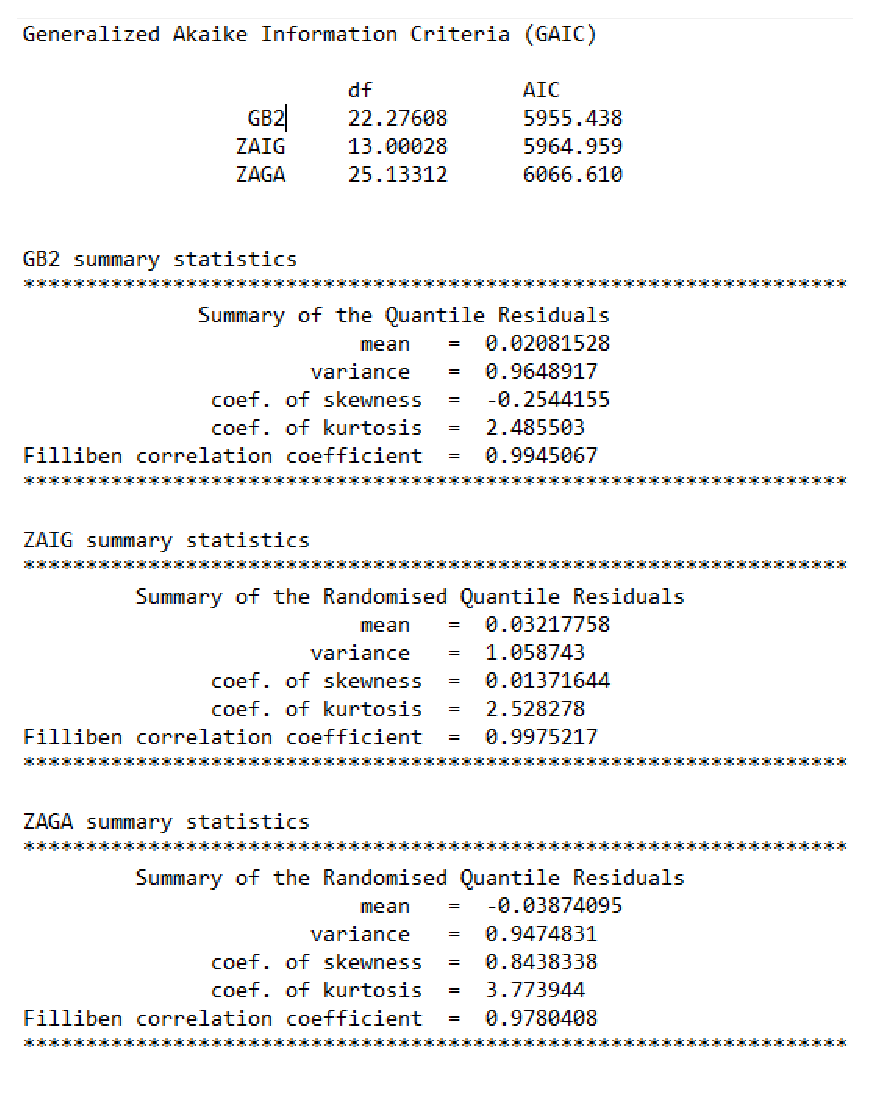
\includegraphics[width=1\linewidth]{GAIC_statistics.eps}
   \caption{}
   \label{Residuals summary statistics} 
\end{subfigure}

\begin{subfigure}[b]{0.5\textwidth}
   \includegraphics[width=1\linewidth]{ROC_4Plot_GB2.eps}
   \caption{}
   \label{Residuals_GB2}
\end{subfigure}

\caption[Normalized quantile residuals from model GB2]{(a)Summary statistics of quantile residuals from models GB2, ZAIG \& ZAGA (b)Displays (normalized quantile) residuals from model $\mbox{GB}2(\mu,\sigma,\nu,\tau)$.}
\end{figure}

\begin{figure}
\centering
\begin{subfigure}[b]{0.5\textwidth}
   \includegraphics[width=1\linewidth]{ROC_4Plot_ZAIG.eps}
   \caption{}
   \label{Residuals_ZAIG} 
\end{subfigure}

\begin{subfigure}[b]{0.5\textwidth}
   \includegraphics[width=1\linewidth]{ROC_4Plot_ZAGA.eps}
   \caption{}
   \label{Residuals_ZAGA}
\end{subfigure}

\caption[Normalized quantile residuals from models ZAIG \& ZAGA]{(a) Display of (normalized quantile) residuals from model $\mbox{ZAIG}(\mu,\sigma,\nu)$ (b) As for (a) but on the model $\mbox{ZAGA}(\mu,\sigma,\nu)$}
\end{figure}

\end{document}
